\section{Introduction}\label{introduction}

In order to classify the research on the different fields related to
software maintenance, we can reason about types of bugs at different
levels. For example, we can group bugs based on the developers that fix
them or using information about the bugs such as crash traces.

There have been several studies (e.g., {[}@Weiß2007; @Zhang2013{]}) that
study of the factors that influence the bug fixing time. These studies
empirically investigate the relationship between bug report attributes
(description, severity, etc.) and the fixing time. Other studies take
bug analysis to another level by investigating techniques and tools for
bug prediction and reproduction (e.g., {[}@Chen2013; @Kim2007a;
@Nayrolles2015{]}). These studies, however, treat all bugs as the same.
For example, a bug that requires only one fix is analyzed the same way
as a bug that necessitates multiple fixes. Similarly, if multiple bugs
are fixed by modifying the exact same locations in the code, then we
should investigate how these bugs are related in order to predict them
in the future. Note here that we do not refer to duplicate bugs.
Duplicate bugs are marked as duplicate (and not fixed) and only the
master bug is fixed. As a motivating example, consider Bugs \#AMQ-5066
and \#AMQ-5092 from the Apache Software Foundation bug report management
system (used to build one of the datasets in this paper). Bug \#AMQ-5066
was reported on February 19, 2014 and solved with a patch provided by
the reporter. The solution involves a relatively complex patch that
modifies \{\tt MQTTProtocolConverter.java\},
\{\tt MQTTSubscription.java\} and \{\tt MQTTTest.java\} files. The
description of the bug is as follows:

\emph{When a client sends a SUBSCRIBE message with the same Topic/Filter
as a previous SUBSCRIBE message but a different QoS, the Server MUST
discard the older subscription, and resend all retained messages limited
to the new Subscription QoS.}

A few months later, another bug, Bug \#AMQ-5092 was reported:

\emph{MQTT protocol converters does not correctly generate unique packet
ids for retained and non-retained publish messages sent to clients.
{[}\ldots{}{]} Although retained messages published on creation of
client subscriptions are copies of retained messages, they must carry a
unique packet id when dispatched to clients. ActiveMQ re-uses the
retained message's packet id, which makes it difficult to acknowledge
these messages when wildcard topics are used. ActiveMQ also sends the
same non-retained message multiple times for every matching subscription
for overlapping subscriptions. These messages also re-use the
publisher's message id as the packet id, which breaks client
acknowledgment.}

This bug was assigned and fixed by a different person than the one who
fixed bug \#AMQ-5066. The fix consists of modifying slightly the same
lines of the code in the exact files used to fix Bug \#AMQ-5066. In
fact, Bug \#5092 could have been avoided altogether if the first
developer provided a more comprehensive fix to \#AMQ-5066 (a task that
is easier said than done). These two bugs are not duplicates since,
according to their description, they deal with different types of
problems and yet they can be fixed by providing a similar patch. In
other words, the failures are different while the root causes (faults in
the code) are more or less the same. From the bug handling perspective,
if we can develop a way to detect such related bug reports during
triaging then we can achieve considerable time saving in the way bug
reports are processed, for example, by assigning them to the same
developers. We also conjecture that detecting such related bugs can help
with other tasks such as bug reproduction. We can reuse the reproduction
of an already fixed bug to reproduce an incoming and related bug.

Our aim is not to improve testing as it is the case in the work of Eldh
{[}@Eldh2001{]} and Hamill et al. {[}@Hamill2014{]}. Our objective is to
propose a classification that can allow researchers in the filed of
mining bug 9 repositiories to use the taxonomy as a new criterion in
triaging, prediction, and reproduction of bugs. By analogy, we can look
at the proposed bug taxonomy in a similar way as the clone taxonomy
presented by Kapser and Godfrey {[}@CoryKapser{]}. The authors proposed
seven types of source code clones and then conducted a case study, using
their classification, on the file system module of the Linux operating
system. This clone taxonomy continues to be used by researchers to build
better approaches for detecting a given clone type and being able to
effectively compare approaches with each other.

We are interested in bugs that share similar fixes. By a fix, we mean a
modification (adding or deleting lines of code) to an exiting file that
is used to solve the bug. With this in mind, the relationship between
bugs and fixes can be modeled using the UML diagram in Figure
\ref{fig:bug-taxo-diag}. The diagram only includes bugs that are fixed.
From this figure, we can think of four instances of this diagram, which
we refer to as bug taxonomy or simply bug types (see Figure
\ref{fig:bug-taxo}).

\begin{figure}[h!]
  \centering
    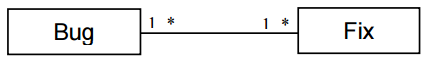
\includegraphics[scale=0.5]{media/bug-taxo-class-diag.png}
    \caption{Class diagram showing the relationship between bugs and fixed
    \label{fig:bug-taxo-diag}}
\end{figure}

\begin{figure}[h!]
  \centering
    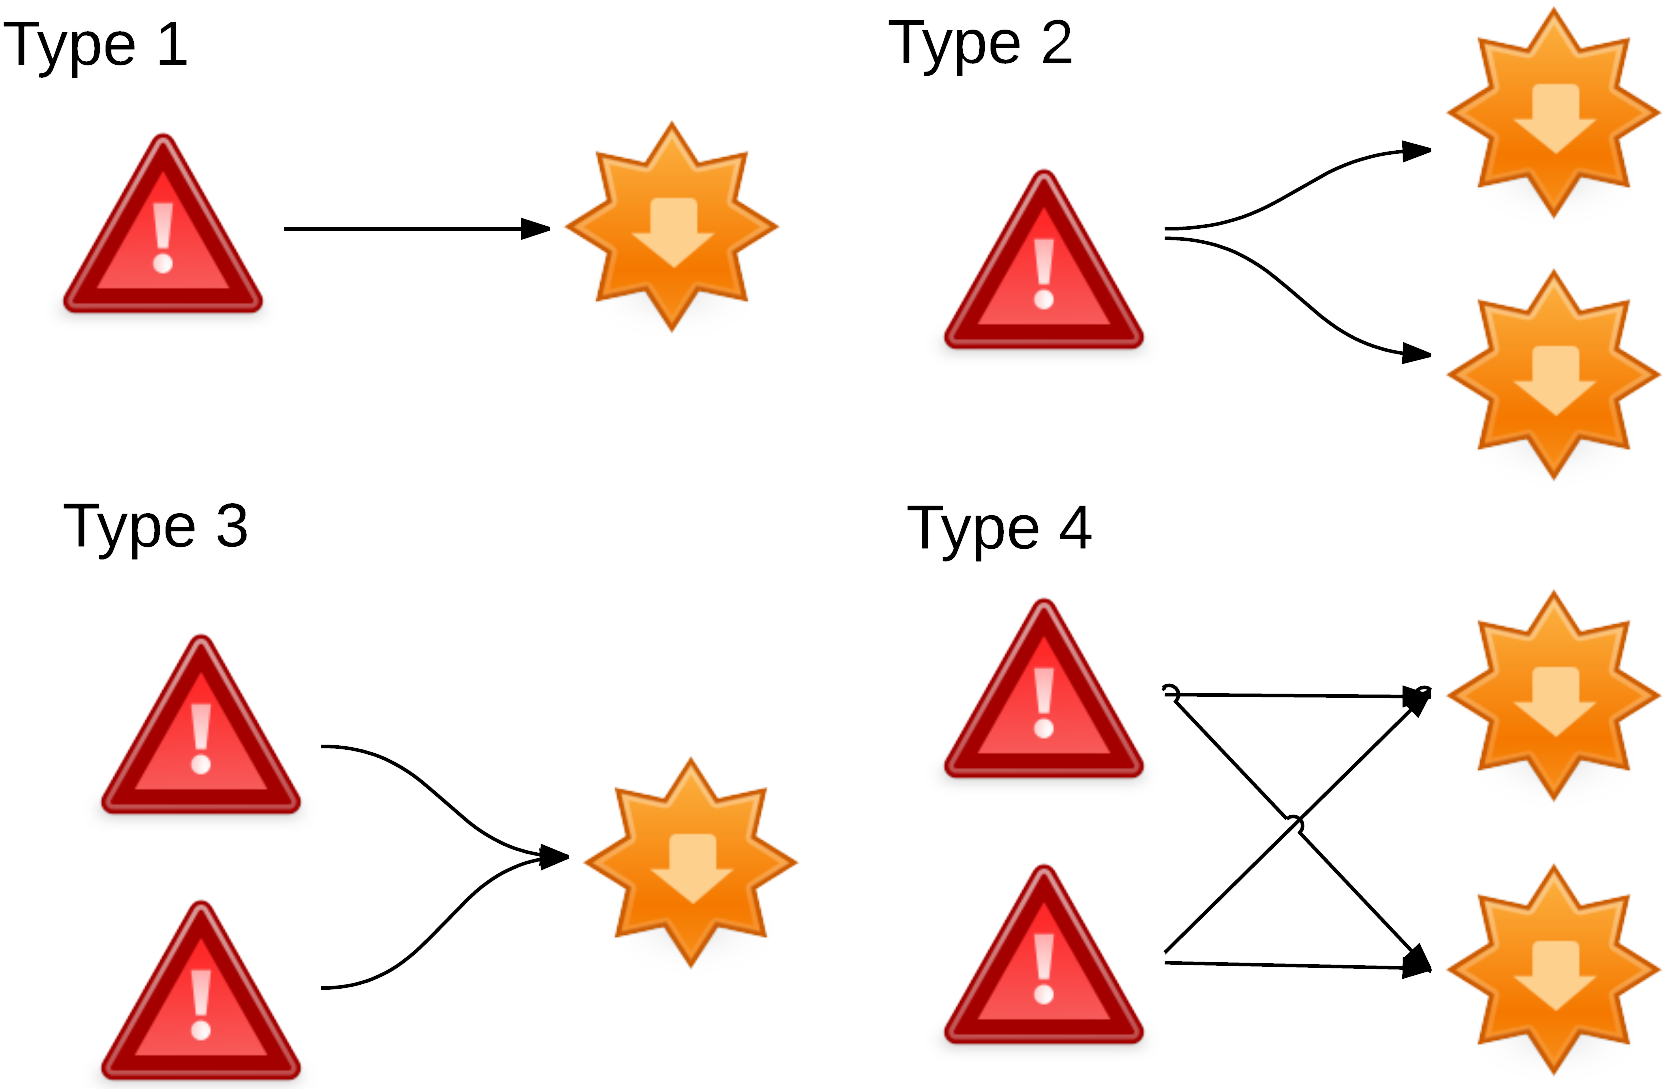
\includegraphics[scale=0.6]{media/bug-taxo.png}
    \caption{Proposed Taxonomy of Bugs
    \label{fig:bug-taxo}}
\end{figure}

The first and second types are the ones we intuitively know about. Type
1 refers to a bug being fixed in one single location (i.e., one file),
while Type 2 refers to bugs being fixed in more than one location. In
Figure 2, only two locations are shown for the sake of clarity, but many
more locations could be involved in the fix of a bug. Type 3 refers to
multiple bugs that are fixed in the exact same location. Type 4 is an
extension of Type 3, where multiple bugs are resolved by modifying the
same set of locations. Note that Type 3 and Type 4 bugs are not
duplicates, they may occur when different features of the system fail
due to the same root causes (faults). We conjecture that knowing the
proportions of each type of bugs in a system may provide insight into
the quality of the system. Knowing, for example, that in a given system
the proportion of Type 2 and 4 bugs is high may be an indication of poor
system quality since many fixes are needed to address these bugs. In
addition, the existence of a high number of Types 3 and 4 bugs calls for
techniques that can effectively find bug reports related to an incoming
bug during triaging. This is similar to the many studies that exist on
detection of duplicates (e.g., {[}@Runeson2007; @Sun2010;
@Nguyen2012{]}), except that we are not looking for duplicates but for
related bugs (bugs that are due to failures of different features of the
system, caused by the same faults). To our knowledge, there is no study
that empirically examines bug data with these types in mind, which is
the main objective of this section. More particularly, we are interested
in the following research questions:

\begin{itemize}
    \item RQ1: What are the proportions of different types of bugs?
    \item RQ2: How complex is each type of bugs?
    \item RQ3: Are bug types predictable at opening time?
\end{itemize}

\section{Study Design}\label{study-design}

The goal of this study is to analyze the location of bug fixes, with the
purpose of classifying bug fixes into types. More specifically, this
study aims to answer the following three research questions:

\begin{itemize}
\item
  \textbf{RQ\(_1\):} \emph{What are the proportions of different types
  of bugs?} This research question aims to what extent bug can be
  classified according to their fix-locations and the proportion of each
  types. Specifically, we investigate if different types of bugs exists
  at all and if the proportion of different types in non-negligible. As
  discussed earlier, knowing, for example, that bugs of Type 3 and 4 are
  the most predominant ones suggests that we need to investigate
  techniques to help detect whether an incoming bug is of Types 3 and 4
  by examining historical data. Similarly, if we can automatically
  identify a bug that is related to another one that has been fixed then
  we can reuse the results of reproducing the first bug in reproducing
  the second one.
\item
  \textbf{RQ\(_2\):} \emph{How complex is each type of bugs?} This
  second research question aims to investigate the complexity of the
  different types of bug. More specifically, we analyze and discuss the
  complexity of different types of bugs using code and process metrics
  both. For the code aspect of the complexity, we compute the number of
  different files impacted by the fix and the number of hunks and
  churns. We do not compute any statistical complexity metrics such as
  cyclomatic complexity {[}@McCabe1989{]}. For the process aspect of
  complexity, we analyze the severity of the bug, the amount of
  duplicate bug report submitted, the number of times a bug report gets
  reopened, the number of comments and the time required to fix the bug.
\item
  \textbf{RQ\(_3\):} \emph{Are bug types predictable at opening time?}
  This third research questions aims at determining the predictability
  of bug types. In details, we investigate what are the best ways to
  predict the type of a bug report at submit time. Being able to build
  accurate classifiers predicting the bug type at submit time will allow
  researcher to enhance triaging approaches. Indeed, combining the
  results of our second research question with an accurate classifier
  will, for example, allow triaging approaches to assign more complex
  bug reports, based on their types, to experienced developers within
  the organization. \#\# Version control
  systems\label{sec:version-control}
\end{itemize}

Version control consists of maintaining the versions of files --- such
as source code and other software artifacts {[}@Zeller1997{]}. This
activity is a complex task and cannot be performed manually on real
world project. Consequently, numerous tools have been created to help
practitioners manage the version of their software artifacts. Each
evolution of a software is a version (or revision) and each version
(revision) is linked to the one before through modifications of software
artifacts. These modifications consist of updating, adding or deleting
software artifacts. They can be referred as \texttt{diff}, \{\tt patch\}
or
\{\tt commit\}\footnote{These names are not to be used interchangeably as difference exists.}.
Each \texttt{diff}, \{\tt patch\} or \{\tt commit\} have the following
characteristics:

\begin{itemize}
\tightlist
\item
  Number of Files: The number of software files that have been modified,
  added or deleted.
\item
  Number of Hunks: The number of consecutive code blocks of modified,
  added or deleted lines in textual files. Hunks are used to determine,
  in each file, how many different places the developer has modified.
\item
  Number of Churns: The number of lines modified. However, the churn
  value for a line change should be at least two as the line has to be
  deleted first and then added back with the modifications.
\end{itemize}

In modern versioning systems, when maintainers make modifications to the
source code want to version it, they have to do commit. The commit
operation will version the modifications applied to one or many files.

Figure \ref{fig:branching} presents the data structure used to store a
commit. Each commit is represented as a tree. The root leaf (green)
contains the commit, tree and parent hashes as same as the author and
the description associated with the commit. The second leaf (blue)
contains the leaf hash and the hashes of the files of the project.

\begin{figure}[h!]
  \centering
    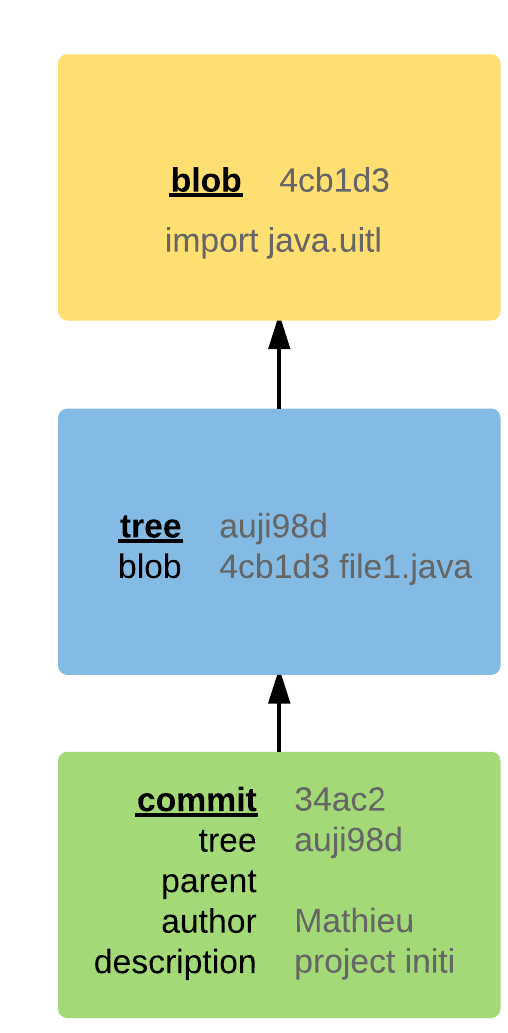
\includegraphics[scale=0.20]{media/commit-datastructure.png}
    \caption{Data structure of a commit.
    \label{fig:branching}}
\end{figure}

In this example, we can see that author
\texttt{Mathieu\textquotesingle{}\textquotesingle{}\ has\ created\ the\ file\ \$file1.java\$\ with\ the\ message}project
init''.

\subsection{Project Tracking Systems\label{sec:issue-tracking}}

Project tracking systems allow end users to create bug reports (BRs) to
report unexpected system behavior, manager can create tasks to drive the
evolution forward and crash report (CRs) can be automatically created.
These systems are also used by development teams to keep track of the
modification induced by bug and to crash reports, and keep track of the
fixes.

\begin{figure}[h!]
    \centering
    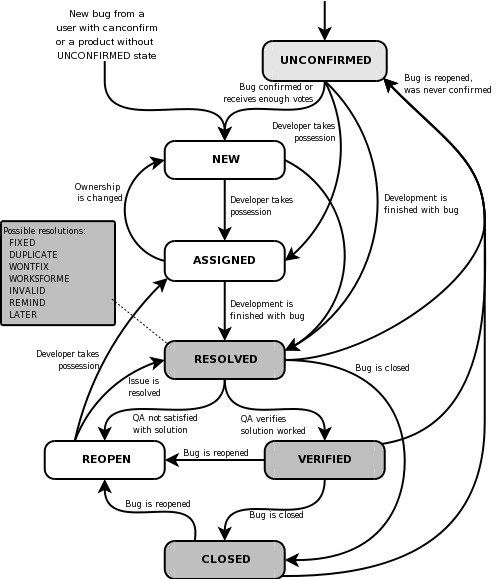
\includegraphics[scale=0.5]{media/bzLifecycle.png}
    \caption{Lifecyle of a report [@Bugzilla2008]}
    \label{fig:bug-lifecyle}
\end{figure}

Figure \ref{fig:bug-lifecyle} presents the life cycle of a report. When
a report is submitted by an end-user, it is set to the
\{\tt UNCONFIRMED\} state until it receives enough votes or that a user
with the proper permissions modifies its status to \{\tt NEW\}. The
report is then assigned to a developer to be fixed. When the report is
in the \{\tt ASSIGNED\} state, the assigned developer(s) starts working
on the report. A fixed report moves to the \{\tt RESOLVED\} state.
Developers have five different possibilities to resolve a report:
\{\tt FIXED\}, \{\tt DUPLICATE\}, \{\tt WONTFIX\}, \{\tt WORKSFORME\}
and \{\tt INVALID\} {[}@Koponen2006{]}.

\begin{itemize}
\tightlist
\item
  \{\tt RESOLVED/FIXED\}: A modification to the source code has been
  pushed, i.e., a changeset (also called a patch) has been committed to
  the source code management system and fixes the root problem described
  in the report.
\item
  \{\tt RESOLVED/DUPLICATE\}: A previously submitted report is being
  processed. The report is marked as duplicate of the original report.
\item
  \{\tt RESOLVED/WONTFIX\}: This is applied in the case where developers
  decide that a given report will not be fixed.
\item
  \{\tt RESOLVED/WORKSFORME\}: If the root problem described in the
  report cannot be reproduced on the reported OS / hardware.
\item
  \{\tt RESOLVED/INVALID\}: If the report is not related to the software
  itself.
\end{itemize}

Finally, the report is \{\tt CLOSED\} after it is resolved. A report can
be reopened (sent to the \{\tt REOPENED\} state) and then assigned again
if the initial fix was not adequate (the fix did not resolve the
problem). The elapsed time between the report marked as the new one and
the resolved status are known as the \{\it fixing time\}, usually in
days. In case of task branching, the branch associated with the report
is marked as ready to be merged. Then, the person in charge (quality
assurance team, manager, ect\ldots{}) will be able to merge the branch
with the mainline. If the report is reopened: the days between the time
the report is reopened and the time it is marked again as
\{\tt RESOLVED/FIXED\} are cumulated. Reports can be reopened many
times.

Tasks follow a similar life cycle with the exception of the
\{\tt UNCONFIRMED\} and \{\tt RESOLVED\} states. Tasks are created by
management and do not need to be confirmed in order to be \{\tt OPEN\}
and \{\tt ASSIGNED\} to developers. When a task is complete, it will not
go to the \{\tt RESOLVED\} state, but to the \{\tt IMPLEMENTED\} state.
Bug and crash reports are considered as problems to eradicate in the
program. Tasks are considered as new features or amelioration to include
in the program.

Reports and tasks can have a severity {[}@Bettenburg2008{]}. The
severity is a classification to indicate the degree of impact on the
software. The possible severities are:

\begin{itemize}
\tightlist
\item
  blocker: blocks development and/or testing work.
\item
  critical: crashes, loss of data, severe memory leak.
\item
  major: major loss of function.
\item
  normal: regular report, some loss of functionality under specific
  circumstances.
\item
  minor: minor loss of function, or other problem where easy workaround
  is present.
\item
  trivial: cosmetic problems like misspelled words or misaligned text.
\end{itemize}

The relationship between an report or a task and the actual modification
can be hard to establish and it has been a subject of various research
studies (e.g., {[}@Antoniol2002; @Bachmann2010; @Wu2011{]}). This reason
is that they are in two different systems: the version control system
and the project tracking system. While it is considered a good practice
to link each report with the versioning system by indicating the report
\(\#id\) on the modification message, more than half of the reports are
not linked to a modification {[}@Wu2011{]}.

\subsection{Context Selection}\label{context-selection}

The context of this study consists of the change history of 388 projects
belonging to two software ecosystem, namely, Apache and Netbeans. Table
\ref{table:datasets} reports, for each of them, (i) the number of
projects analyzed, (ii) size ranges in terms of the number of classes
and KLOC, (iii) the overall number of commits and issues analyzed, and
(iv) the average, minimum, and maximum length of the projects' story (in
years).

\begin{table}[h]
\begin{center}
\begin{tabular}{@{}c|c|c|c|c@{}}
\textbf{Dataset} & \textbf{R/F BR} & \textbf{CS} & \textbf{Files} & \textbf{Projects} \\ \hline \hline
Netbeans         & 53,258          & 122,632     & 30,595         & 39                \\
Apache           & 49,449          & 106,366     & 38,111         & 349               \\
Total            & 102,707         & 229,153     & 68,809         & 388               \\ \hline \hline

\end{tabular}
\end{center}

\caption{Datasets\label{table:datasets}}
\end{table}

All the analyzed projects are hosted in \{\it Git\} or \{\it Mercurial\}
repositories and have either a \{\it Jira\} or a \{\it Bugzilla\} issue
tracker associated with it. The Apache ecosystem consists in 349
projects written in various programming languages (C, C++, Java, Python,
\ldots{}) and uses \{\it Git\} and \{\it Jira\}. These projects
represent the Apache ecosystem in its entirety; no system has been
excluded from our study. The complete list can be found
online\footnote{https://projects.apache.org/projects.html?name}. The
Netbeans ecosystem consists in 39 projects, mostly written in Java.
Similarly to the Apache ecosystem, we did not select any of the projects
belonging to the Netbeans ecosystem but all of them. The Netbeans
community uses \{\it Bugzilla\} and \{\it Mercurial\}.

The choice of the ecosystems to analyze is not random, but rather driven
by the motivation to consider projects having (i) different sizes, (ii)
different architectures, and (iii) different development bases and
processes. Indeed, Apache projects are extremely various in terms of
size of the development team, purpose and technical choices
{[}@Bavota2013{]}. On the other side, Netbeans has a relatively stable
list of core developer and a common vision shared through the 39 related
projects {[}@Wang2011{]}.

Cumulatively, these datasets span from 2001 to 2014. In summary, our
consolidated dataset contains 102,707 bugs, 229,153 changesets, 68,809
files that have been modified to fix the bugs, 462,848 comments, and 388
distinct systems. We also collected 221 million lines of code modified
to fix the bugs, identified 3,284 sub-projects, and 17,984 unique
contributors to these bug report and source code version management
systems. The cumulated opening time for all the bugs reaches 10,661
working years (3,891,618 working days).

\subsection{Data Extraction and
Analysis}\label{data-extraction-and-analysis}

This subsection describes the data extraction and analysis process that
we followed to answer our research questions.

\subsubsection{What are the proportions of different types of
bugs?}\label{what-are-the-proportions-of-different-types-of-bugs}

To answer \textbf{RQ\(_1\)}, we cloned the 349 \{\it git\} repositories
belonging to the Apache ecosystem and the 39 \{\it mercurial\}
repositories belonging to the Netbeans ecosystem. The raw size of the
cloned source code alone, excluding binaries, images and other non-text
file, is 163 GB. Then, we extracted all the 102,707 closed issues that
have been resolved using the \{\it RESOLVED/FIXED\} tags. Indeed, this
study aims to classify bugs according to their fix locations. If an
issue is fixed by other means than \{\it fixing\} the source code, then,
it falls outside the scope our study. In order to assign commits to
issues we used is the regular expression-based approach by Fischer et
al. {[}@Fischer{]} matching the issue ID in the commit note. Using this
technique, we were able to link almost 40\% (40,493 out of 102,707) of
our resolved/fixed issues to 229,153 commits. An issue can be fixed with
several commits.

We choose not to use more complex technics like ReLink, an approach
proposed by Wu et al.{[}@Wu2011{]}, which considers the following
constraints: (i) matching the committer/authors with issue tracking
contributor name/email; (ii) the time interval between the commit and
the last comment posted by the same author/contributor on the issue
tracker must be less than seven days; and (iii) Vector Space Model (VSM)
cosine similarity between the commit note and the last comment referred
above or greater than 0.7 because we believe that mining more than forty
thousands issues is enough to be significant.

Using our generated consolidated dataset, we extracted the files \(f_i\)
impacted by each commit \(c_i\) for each one of our 388 projects. Then,
we classify the bugs according to the following:

\begin{itemize}
\tightlist
\item
  \textbf{Type 1:} A bug is tagged type 1 if it is fixed by modifying a
  file \(f_i\) and \(f_i\) is not involved in any other bug fix.
\item
  \textbf{Type 2:} A bug is tagged type 2 if it is fixed by modifying
  several files \(f_{i..n}\) and the files \(f_{i..n}\) are not involved
  in any other bug fix.
\item
  \textbf{Type 3:} A bug is tagged type 3 if it is fixed by modifying a
  file \(f_{i}\) and the file \(f_{i}\) is involved in fixing other
  bugs.
\item
  \textbf{Type 4:} A bug is tagged type 4 if it is fixed by modifying
  several files \(f_{i..n}\) and the files \(f_{i..n}\) are involved in
  any other bug fix.
\end{itemize}

To answer this question, we analyze whether any type is predominant in
the studied ecosystem, by testing the null hypothesis:

\begin{itemize}
\tightlist
\item
  \(H_{01}\) : The proportion of types does not change significantly
  across the studied ecosystems.
\end{itemize}

We test this hypothesis by observing both a `'global'`(across ecosystem)
and a'`local'' predominance (per ecosystem) of the different types of
bugs. We must observe these two aspects to ensure that the predominance
of a particular type of bug is not circumstantial (in few given systems
only) but is also not due to some other, unknown factors (in all systems
but not in a particular ecosystem).

We answer \textbf{RQ\(_1\)} in two steps. The first step is to use
descriptive statistics; we compute the ratio of each types to the total
number of bugs in the dataset.

In the second step, we compare the proportions of the different types of
bugs with respect to the ecosystem where the bugs were found. We build
the contingency table with these two qualitative variables (the type and
studied ecosystem) and test the null hypothesis \textbf{H\(_{01A}\)} to
assess whether the proportion of a particular type of bugs is related to
a specific ecosystem or not.

We use the Pearson's chi-squared test to reject the null hypothesis
\(H_{01A}\). Pearson's chi-squared independence test is used to analyze
the relationship between two qualitative data, in our study the type
bugs and the studied ecosystem. The results of Pearson's chi-squared
independence tests are considered statistically significant at
\(\alpha\) = 0.05. If p-value \(\le\) 0.05, we reject the null
hypothesis \(H_{01A}\) and conclude that the proportion of each types is
different for each ecosystem.

Overall, the data extraction and manipulation for \textbf{RQ\(_1\)}
(i.e., cloning repositories, linking commits to issues and tagging
issues by type) took thirteen weeks on two Linux servers having 1
quadcore 3.10 GHz CPU and 12 GB of RAM each.

\subsubsection{How complex is each type of
bugs?}\label{how-complex-is-each-type-of-bugs}

To answer \textbf{RQ\(_2\)} we went through the 40,493 resolved/fixed
issues and the linked 229,153 commits in order to compute code and
process metrics for each of them. These metrics will then be used to
assess the complexity of a bug. The computed process metrics are:

\begin{itemize}
\tightlist
\item
  The time \(t\) it took to resolve issue \(i\).
\item
  The number of issues \(dup\) tagged as duplicate of issue \(i\).
\item
  The number of time issue \(i\) got reopen \(reop\).
\item
  The number of comments \(comment\) on issue \(i\).
\item
  The severity \(sev\) of the issue \(i\).
\end{itemize}

The computed code metrics are:

\begin{itemize}
\tightlist
\item
  The number of files \(f\) impacted by issue \(i\).
\item
  The number of commit \(c\) required to fix the issue \(i\).
\item
  The number of hunks \(h\) required to fix the issue \(i\).
\item
  The number of churns \(ch\) required to fix the issue \(i\).
\end{itemize}

We address the relation between types and the complexity of the bugs in
using our metrics. We analyze whether Types 2 and 4 bugs are more
complex to handle than Types 1 and 3 bugs, by testing the null
hypotheses:

\begin{itemize}
\tightlist
\item
  \(H_{02}\): The complexity of bug types is not significantly different
  from type to type.
\end{itemize}

To test our hypothesis, we build a contingency table with the
qualitative variables and the dependent variable for each type.

We use the Pearson's chi-squared test to reject the null hypothesis
\(H_{02}\). The results of Pearson's chi-squared independence tests are
considered statistically significant at \(\alpha\) = 0.05. If a p-value
\(\le\) 0.05, we reject the null hypothesis \(H_{02}\) and conclude that
the complexity of bug is related to its type.

\subsubsection{Are bug types predictable at opening
time?}\label{are-bug-types-predictable-at-opening-time}

This third research question aims at determining the predictability of
bug types. In details, we investigate what are the best ways to predict
the type of a bug report at submit time. Being able to build accurate
classifiers predicting the bug type at submit time will allow researcher
to enhance triaging approaches. Indeed, combining the results of our
second research question with an accurate classifier will, for example,
allow triaging approaches to assign more complex bug reports, based on
their types, to experienced developers within the organization. In order
to answer this question we used the text contained on the bug report and
the text from the comment posted the first 48 hours after the report's
opening as they are likely to give some additional information about the
bug itself. Then, we removed all the stopwords (i.e.~the, or, she, he)
and truncated the remaining words to their roots (i.e.~writing becomes
write, failure becomes fail and so on). Finally, we apply the compute
tfidf on the transformed text and create three different datasets using
the n-grams technique. The datasets are 1, 2 and 3-grams. In order to
build the classifier, we use three well-known machine learning
techniques that are proven to yield satisfactory results while working
on bug reports: svm, random forest and linear regression.

We analyze whether bug types are predictable by testing the null
hypothesis:

\begin{itemize}
\tightlist
\item
  \(H_{03}\): Bug types classifiers are not accurate.
\end{itemize}

To test our hypothesis, we predict the bug type of the most complex
type, according to \textbf{RQ\(_2\)}, in ten different projects.

\subsection{Analysis of the Results}\label{analysis-of-the-results}

This section reports the analysis of the results aiming at answering our
three research questions.

\subsubsection{What are the proportions of different types of
bugs?}\label{what-are-the-proportions-of-different-types-of-bugs-1}

\begin{table*}[]
\centering
\small
\caption{Contingency table and Pearson's chi-squared tests}
\label{tab:contingency-table}
\resizebox{\textwidth}{!}{%
\begin{tabular}{cccccc}
Ecosystem & T1                 & T2               & T3                & T4                & Pearson's chi-squared p-Value                          \\ \rowcolor{gray!25}
Apache    & 1968  (14.3 \%)   & 1248  (9.1 \%)  & 3101  (22.6 \%)  &7422  ( 54 \%)    &  \\ \rowcolor{gray!25}
Netbeans  & 776  (2.9 \%)     & 240  (0.9 \%)   & 8372  (31.3 \%)  & 17366  (64.9 \%) &  \textless0.01                               \\ \rowcolor{gray!25}
Overall   & 2744  (6.8 \%)    & 1488  (3.7 \%)  & 11473  (28.3 \%) & 24788  (61.2 \%) &                                \\
\end{tabular}
}
\end{table*}


Table \ref{tab:contingency-table} presents a contingency table and the
results of the Pearson's chi-squared tests we performed on each types of
bug. In addition to presenting bug types 1 to 4, Table
\ref{tab:contingency-table} also presents grouping of bug types: Types 1
and 2 versus Types 3 and 4.

Types 3 (22.6\% and 54\%) and 4 (31.3\% and 64.9\%) are predominant
compared to types 1 (14.3\% and 9.1\%) and 2 (6.8\% and 3.7\%) for the
Apache and the Netbeans ecosystems, respectively. Overall, the
proportion of different types of bug is as follows: 6.8\%, 3.7\%,
28.3\%, 61.2\% for types 1, 2, 3 and 4, respectively. The result of the
Pearson's test is below 0.01. As a reminder, we consider results of
Pearson's tests statistically significant at \(\alpha \textless0.05\).
Consequently, we reject to null hypothesis \(H_{01}\) and conclude that
there is a predominance of Types 3 and 4 in all different ecosystems and
this observation is not related to a specific ecosystem. When combined
into our first group, Types 1 \& 2 versus Types 3 \& 4, there are
significantly more Types 3 and 4 (89.5 \%) than Types 1 and 2 (10.5 \%).

\subsubsection{How complex is each type of
bugs?}\label{how-complex-is-each-type-of-bugs-1}

To answer \{\bf RQ$_2$\}, we analyze the complexity of each bug in terms
of duplication, fixing time, comments, reopenning, files impacted,
severity, changesets, hunks and chunks.

Figure \ref{fig:boxplots} presents nine boxplots describing our
complexity metric for each type of each ecosystem. In each sub-figure,
the book plates are organized as follows: (a) Types 1 to 4 bugs for the
Apache ecosystem, (b) Types 1 to 4 bugs for the Netbeans ecosystem and
(c) Types 1 to 4 bugs for both ecosystems combined. For all the metrics,
except the severity, the median is close to zero and we can observe many
outliers. Tables \ref{tab:apache-eco}, \ref{tab:netbeans-eco} and
\ref{tab:overall-eco} present descriptive statistics about each metric
for each type for the Apache ecosystem, the Netbeans ecosystem, and both
ecosystems combined, respectively. The descriptive statistics used are
\(\mu\):mean, \(\sum\):sum, \(\hat{x}\):median, \(\sigma\):standard
deviation and \(\%\):percentage. In addition, to the descriptive
statistics, these tables present matrices of Mann-Whitney test for each
metric and type. We added the \checkmark\textasciitilde{}symbol to the
Mann-Whitney tests results columns when the value is statistically
significant (e.g. \(\alpha \textless 0.05\)) and
\xmark\textasciitilde{}otherwise.

Finally, Table \ref{tab:chi-rq2} presents the Pearson's chi-squared test
results for each complexity metric for Types 1 to 4 and our two types
combination. In what follows, we present our findings for each
complexity metric. Complexity metrics are divided into two groups: (a)
process and (b) code metrics. Process metrics refer to metrics that have
been extracted from the project tracking system (i.e., fixing time,
comments, reopening and severity). Code metrics are directly computed
using the source code used to fix a given bug (i.e., files impacted,
changesets required, hunks and chunks). We acknowledge that these
complexity metrics only represent an abstraction of the actual
complexity of a given bug as they cannot account for the actual thought
process and expertise required to craft a fix. However, we believe that
they are an accurate abstraction. Moreover, they are used in several
studies in the field to approximate the complexity of a bug
\cite{Weiß2007,Saha2014,Nam2013,Anvik2006,Nagappan}.

\textbackslash{}begin\{figure*\} \centering
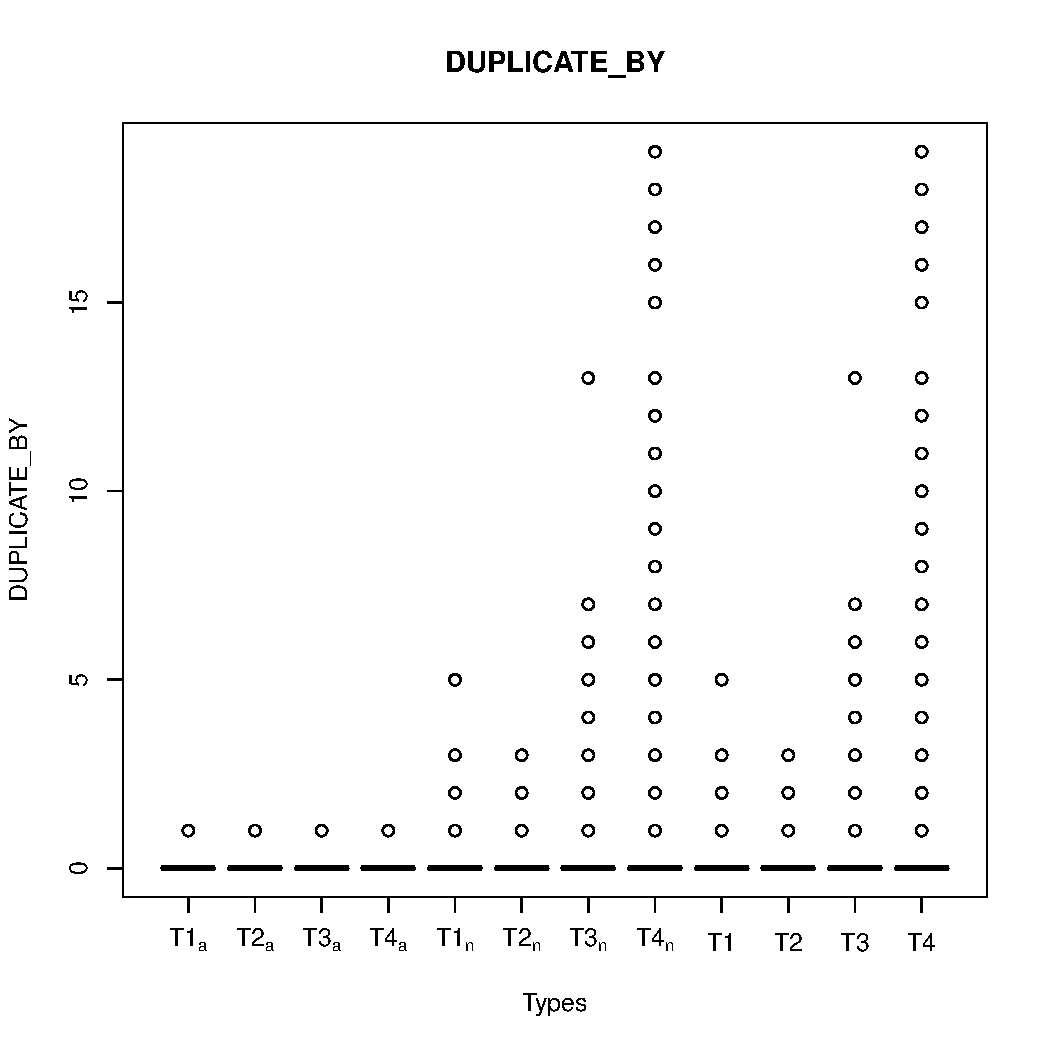
\includegraphics[page=1, width=0.45\textwidth]{extract/Rplots}
\includegraphics[page=2, width=0.45\textwidth]{extract/Rplots}
\textbackslash{}
\includegraphics[page=3, width=0.45\textwidth]{extract/Rplots}
\includegraphics[page=4, width=0.45\textwidth]{extract/Rplots}
\textbackslash{}
\includegraphics[page=5, width=0.45\textwidth]{extract/Rplots}
\includegraphics[page=6, width=0.45\textwidth]{extract/Rplots}

\label{fig:boxplots}\}

\textbackslash{}end\{figure*\}

\begin{figure*}
\centering
\includegraphics[page=7, width=0.45\textwidth]{extract/Rplots}
\includegraphics[page=8, width=0.45\textwidth]{extract/Rplots} \\
\includegraphics[page=9, width=0.45\textwidth]{extract/Rplots}

\caption{Complexity metrics boxplots. From left to right and top to bottom: Duplicate, Fixing time, Comments, Reopening, Files impacted, Severity, Changesets, Hunks and Chunks.
\label{fig:boxplots}}

\end{figure*}

%!TEX root = ..bug-taxo.tex

% Please add the following required packages to your document preamble:
% \usepackage{graphicx}
\begin{table*}[]
\centering
\samll
\setlength\extrarowheight{6pt}
\caption{My caption}
\label{my-label}
\begin{tabular}{ccccccc|ccccc}

Types & Metric &$^\mu$ & $^\sum$ & $^\hat{x}$ & $^\sigma$ & $^\%$ & T1 & T2 & T3 & T4 \\ \hline \rowcolor{gray!25}
& Dup. & 0.026 & 51 & 0 & 0.2 & 14.8 & n.a & \xmark (0.53) & \checkmark  (\textless 0.05) & \xmark (0.45)  \\ \rowcolor{gray!25}
& Tim. & 91.574 & 180217 & 4 & 262 & 21.8 & n.a & \checkmark  (\textless 0.05) & \checkmark  (\textless 0.05) & \checkmark  (\textless 0.05)  \\ \rowcolor{gray!25}
& Com. & 4.355 & 8571 & 3 & 4.7 & 9.5 & n.a & \checkmark  (\textless 0.05) & \xmark (0.17) & \checkmark  (\textless 0.05)  \\ \rowcolor{gray!25}
& Reo. & 0.062 & 122 & 0 & 0.3 & 13.8 & n.a & \xmark (0.29) & \checkmark  (\textless 0.05) & \checkmark  (\textless 0.05)  \\ \rowcolor{gray!25}
T1 & Fil. & 0.991 & 1950 & 1 & 0.1 & 3.7 & n.a & \checkmark  (\textless 0.05) & \xmark (0.28) & \checkmark  (\textless 0.05)  \\ \rowcolor{gray!25}
& Sev. & 3.423 & 6737 & 4 & 1.3 & 13.2 & n.a & \xmark (0.18) & \checkmark  (\textless 0.05) & \checkmark  (\textless 0.05)  \\ \rowcolor{gray!25}
& Cha. & 1 & 1968 & 1 & 0 & 1.9 & n.a & \checkmark  (\textless 0.05) & \checkmark  (\textless 0.05) & \checkmark  (\textless 0.05)  \\ \rowcolor{gray!25}
& Hun. & 3.814 & 7506 & 3 & 2.4 & 0 & n.a & \checkmark  (\textless 0.05) & \checkmark  (\textless 0.05) & \checkmark  (\textless 0.05)  \\ \rowcolor{gray!25}
& Chur. & 18.761 & 36921 & 7 & 48.6 & 0 & n.a & \checkmark  (\textless 0.05) & \xmark (0.09) & \checkmark  (\textless 0.05)  \\


 & Dup. & 0.022 & 28 & 0 & 0.1 & 8.1 & \xmark (0.53) & n.a & \xmark (0.16) & \xmark (0.19)  \\
 & Tim. & 115.158 & 143717 & 8 & 294.1 & 17.4 & \checkmark  (\textless 0.05) & n.a & \checkmark  (\textless 0.05) & \checkmark  (\textless 0.05)  \\
 & Com. & 5.041 & 6291 & 4 & 4.7 & 7 & \checkmark  (\textless 0.05) & n.a & \checkmark  (\textless 0.05) & \checkmark  (\textless 0.05)  \\
 & Reo. & 0.071 & 89 & 0 & 0.3 & 10.1 & \xmark (0.29) & n.a & \checkmark  (\textless 0.05) & \xmark (0.59)  \\
T2 & Fil. & 4.381 & 5468 & 2 & 20.4 & 10.5 & \checkmark  (\textless 0.05) & n.a & \checkmark  (\textless 0.05) & \checkmark  (\textless 0.05)  \\
 & Sev. & 3.498 & 4365 & 4 & 1.2 & 8.6 & \xmark (0.18) & n.a & \checkmark  (\textless 0.05) & \checkmark  (\textless 0.05)  \\
 & Cha. & 4.681 & 5842 & 2 & 20.4 & 5.5 & \checkmark  (\textless 0.05) & n.a & \checkmark  (\textless 0.05) & \checkmark  (\textless 0.05)  \\
 & Hun. & 561.995 & 701370 & 14 & 13628.2 & 3.9 & \checkmark  (\textless 0.05) & n.a & \checkmark  (\textless 0.05) & \checkmark  (\textless 0.05)  \\
 & Chur. & 14184.869 & 17702716 & 88 & 400710.2 & 8 & \checkmark  (\textless 0.05) & n.a & \checkmark  (\textless 0.05) & \checkmark  (\textless 0.05)  \\

 \rowcolor{gray!25}
 & Dup. & 0.016 & 50 & 0 & 0.1 & 14.5 & \checkmark  (\textless 0.05) & \xmark (0.16) & n.a & \checkmark  (\textless 0.05)  \\ \rowcolor{gray!25}
 & Tim. & 35.892 & 111300 & 1 & 151.8 & 13.5 & \checkmark  (\textless 0.05) & \checkmark  (\textless 0.05) & n.a & \checkmark  (\textless 0.05)  \\ \rowcolor{gray!25}
 & Com. & 4.422 & 13712 & 3 & 4.4 & 15.2 & \xmark (0.17) & \checkmark  (\textless 0.05) & n.a & \checkmark  (\textless 0.05)  \\ \rowcolor{gray!25}
 & Reo. & 0.033 & 101 & 0 & 0.2 & 11.5 & \checkmark  (\textless 0.05) & \checkmark  (\textless 0.05) & n.a & \checkmark  (\textless 0.05)  \\ \rowcolor{gray!25}
 T3 & Fil. & 0.994 & 3081 & 1 & 0.1 & 5.9 & \xmark (0.28) & \checkmark  (\textless 0.05) & n.a & \checkmark  (\textless 0.05)  \\ \rowcolor{gray!25}
 & Sev. & 3.644 & 11300 & 4 & 1.1 & 22.2 & \checkmark  (\textless 0.05) & \checkmark  (\textless 0.05) & n.a & \checkmark  (\textless 0.05)  \\ \rowcolor{gray!25}
 & Cha. & 1 & 3101 & 1 & 0 & 2.9 & \checkmark  (\textless 0.05) & \checkmark  (\textless 0.05) & n.a & \checkmark  (\textless 0.05)  \\ \rowcolor{gray!25}
 & Hun. & 4.022 & 12472 & 3 & 3.4 & 0.1 & \checkmark  (\textless 0.05) & \checkmark  (\textless 0.05) & n.a & \checkmark  (\textless 0.05)  \\ \rowcolor{gray!25}
 & Chur. & 16.954 & 52573 & 6 & 49.8 & 0 & \xmark (0.09) & \checkmark  (\textless 0.05) & n.a & \checkmark  (\textless 0.05)  \\


& Dup. & 0.029 & 216 & 0 & 0.2 & 62.6 & \xmark (0.45) & \xmark (0.19) & \checkmark  (\textless 0.05) & n.a  \\
& Tim. & 52.76 & 391586 & 4 & 182.2 & 47.4 & \checkmark  (\textless 0.05) & \checkmark  (\textless 0.05) & \checkmark  (\textless 0.05) & n.a  \\
& Com. & 8.313 & 61701 & 5 & 10.2 & 68.3 & \checkmark  (\textless 0.05) & \checkmark  (\textless 0.05) & \checkmark  (\textless 0.05) & n.a  \\
& Reo. & 0.077 & 570 & 0 & 0.3 & 64.6 & \checkmark  (\textless 0.05) & \xmark (0.59) & \checkmark  (\textless 0.05) & n.a  \\
T4 & Fil. & 5.633 & 41805 & 3 & 14 & 79.9 & \checkmark  (\textless 0.05) & \checkmark  (\textless 0.05) & \checkmark  (\textless 0.05) & n.a  \\
& Sev. & 3.835 & 28466 & 4 & 1 & 56 & \checkmark  (\textless 0.05) & \checkmark  (\textless 0.05) & \checkmark  (\textless 0.05) & n.a  \\
& Cha. & 12.861 & 95455 & 4 & 52.2 & 89.7 & \checkmark  (\textless 0.05) & \checkmark  (\textless 0.05) & \checkmark  (\textless 0.05) & n.a  \\
& Hun. & 2305.868 & 17114149 & 30 & 58094.7 & 96 & \checkmark  (\textless 0.05) & \checkmark  (\textless 0.05) & \checkmark  (\textless 0.05) & n.a  \\
& Chur. & 27249.773 & 202247816 & 204 & 320023.5 & 91.9 & \checkmark  (\textless 0.05) & \checkmark  (\textless 0.05) & \checkmark  (\textless 0.05) & n.a

\end{tabular}%
\end{table*}
 %!TEX root = ..bug-taxo.tex

\begin{table*}[]
\centering
\small
\setlength\extrarowheight{6pt}
\caption{My caption}
\label{my-label}
\begin{tabular}{ccccccc|ccccc}

Types & Metric &$^\mu$ & $^\sum$ & $^\hat{x}$ & $^\sigma$ & $^\%$ & T1 & T2 & T3 & T4 \\ \hline \rowcolor{gray!25}

& Dup. & 0.086 & 67 & 0 & 0.4 & 2.5 & n.a & \xmark (0.39) & \xmark (0.24) & \xmark (0.86) \\  \rowcolor{gray!25}
& Tim. & 92.759 & 71981 & 10 & 219.1 & 2.3 & n.a & \checkmark  (\textless 0.05) & \xmark (0.15) & \checkmark  (\textless 0.05) \\  \rowcolor{gray!25}
& Com. & 4.687 & 3637 & 3 & 4.1 & 2.4 & n.a & \checkmark  (\textless 0.05) & \xmark (0.83) & \checkmark  (\textless 0.05)  \\  \rowcolor{gray!25}
& Reo. & 0.054 & 42 & 0 & 0.3 & 1.9 & n.a & \xmark (0.1) & \xmark (0.58) & \checkmark  (\textless 0.05)  \\  \rowcolor{gray!25}
T1 & Fil. & 1.735 & 1346 & 1 & 13.2 & 0.8 & n.a & \checkmark  (\textless 0.05) & \checkmark  (\textless 0.05) & \checkmark  (\textless 0.05)  \\  \rowcolor{gray!25}
& Sev. & 4.314 & 3348 & 3 & 1.5 & 3.1 & n.a & \xmark (0.66) & \checkmark  (\textless 0.05) & \checkmark  (\textless 0.05)  \\  \rowcolor{gray!25}
& Cha. & 1.085 & 842 & 1 & 0.4 & 2 & n.a & \xmark (0.99) & \xmark (0.26) & \checkmark  (\textless 0.05)  \\  \rowcolor{gray!25}
& Hun. & 4.405 & 3418 & 3 & 7 & 0.5 & n.a & \checkmark  (\textless 0.05) & \xmark (0.13) & \checkmark  (\textless 0.05)  \\  \rowcolor{gray!25}
& Chur. & 5.089 & 3949 & 2 & 12.5 & 0.3 & n.a & \checkmark  (\textless 0.05) & \checkmark  (\textless 0.05) & \checkmark  (\textless 0.05)  \\


 & Dup. & 0.067 & 16 & 0 & 0.3 & 0.6 & \xmark (0.39) & n.a & \xmark (0.73) & \xmark (0.39) \\
 & Tim. & 111.9 & 26856 & 16 & 308.6 & 0.9 & \checkmark  (\textless 0.05) & n.a & \checkmark  (\textless 0.05) & \xmark (0.41) \\
 & Com. & 4.433 & 1064 & 3 & 4 & 0.7 & \checkmark  (\textless 0.05) & n.a & \checkmark  (\textless 0.05) & \checkmark  (\textless 0.05) \\
 & Reo. & 0.079 & 19 & 0 & 0.3 & 0.9 & \xmark (0.1) & n.a & \xmark (0.11) & \xmark (0.97) \\
T2 & Fil. & 8.804 & 2113 & 2 & 42.7 & 1.3 & \checkmark  (\textless 0.05) & n.a & \checkmark  (\textless 0.05) & \checkmark  (\textless 0.05) \\
 & Sev. & 4.362 & 1047 & 3 & 1.5 & 1 & \xmark (0.66) & n.a & \checkmark  (\textless 0.05) & \checkmark  (\textless 0.05) \\
 & Cha. & 1.075 & 258 & 1 & 0.3 & 0.6 & \xmark (0.99) & n.a & \xmark (0.5) & \checkmark  (\textless 0.05)  \\
 & Hun. & 21.887 & 5253 & 8 & 62.7 & 0.7 & \checkmark  (\textless 0.05) & n.a & \checkmark  (\textless 0.05) & \checkmark  (\textless 0.05) \\
 & Chur. & 32.263 & 7743 & 8 & 125.8 & 0.7 & \checkmark  (\textless 0.05) & n.a & \checkmark  (\textless 0.05) & \checkmark  (\textless 0.05)  \\

 \rowcolor{gray!25}
& Dup. & 0.074 & 620 & 0 & 0.4 & 23.3 & \xmark (0.24) & \xmark (0.73) & n.a & \checkmark  (\textless 0.05)  \\  \rowcolor{gray!25}
& Tim. & 87.033 & 728642 & 9 & 233.6 & 23.8 & \xmark (0.15) & \checkmark  (\textless 0.05) & n.a & \checkmark  (\textless 0.05) \\  \rowcolor{gray!25}
& Com. & 4.73 & 39599 & 3 & 4.3 & 26.5 & \xmark (0.83) & \checkmark  (\textless 0.05) & n.a & \checkmark  (\textless 0.05)  \\  \rowcolor{gray!25}
& Reo. & 0.06 & 499 & 0 & 0.3 & 22.7 & \xmark (0.58) & \xmark (0.11) & n.a & \checkmark  (\textless 0.05)  \\  \rowcolor{gray!25}
T3 & Fil. & 1.306 & 10932 & 1 & 5.1 & 6.8 & \checkmark  (\textless 0.05) & \checkmark  (\textless 0.05) & n.a & \checkmark  (\textless 0.05) \\  \rowcolor{gray!25}
& Sev. & 4.021 & 33666 & 3 & 1.4 & 31.4 & \checkmark  (\textless 0.05) & \checkmark  (\textless 0.05) & n.a & \checkmark  (\textless 0.05) \\  \rowcolor{gray!25}
& Cha. & 1.065 & 8917 & 1 & 0.3 & 21 & \xmark (0.26) & \xmark (0.5) & n.a & \checkmark  (\textless 0.05) \\  \rowcolor{gray!25}
& Hun. & 5.15 & 43115 & 3 & 12.4 & 5.8 & \xmark (0.13) & \checkmark  (\textless 0.05) & n.a & \checkmark  (\textless 0.05) \\  \rowcolor{gray!25}
& Chur. & 6.727 & 56317 & 2 & 22 & 4.9 & \checkmark  (\textless 0.05) & \checkmark  (\textless 0.05) & n.a & \checkmark  (\textless 0.05)  \\


 & Dup. & 0.113 & 1959 & 0 & 0.7 & 73.6 & \xmark (0.86) & \xmark (0.39) & \checkmark  (\textless 0.05) & n.a \\
 & Tim. & 128.833 & 2237319 & 13 & 332.8 & 73 & \checkmark  (\textless 0.05) & \xmark (0.41) & \checkmark  (\textless 0.05) & n.a \\
 & Com. & 6.058 & 105202 & 4 & 6.7 & 70.4 & \checkmark  (\textless 0.05) & \checkmark  (\textless 0.05) & \checkmark  (\textless 0.05) & n.a \\
 & Reo. & 0.094 & 1639 & 0 & 0.4 & 74.5 & \checkmark  (\textless 0.05) & \xmark (0.97) & \checkmark  (\textless 0.05) & n.a & \\
T4 & Fil. & 8.408 & 146019 & 4 & 25.1 & 91 & \checkmark  (\textless 0.05) & \checkmark  (\textless 0.05) & \checkmark  (\textless 0.05) & n.a \\
 & Sev. & 3.982 & 69159 & 3 & 1.4 & 64.5 & \checkmark  (\textless 0.05) & \checkmark  (\textless 0.05) & \checkmark  (\textless 0.05) & n.a \\
 & Cha. & 1.871 & 32494 & 2 & 1.2 & 76.4 & \checkmark  (\textless 0.05) & \checkmark  (\textless 0.05) & \checkmark  (\textless 0.05) & n.a \\
 & Hun. & 40.195 & 698022 & 13 & 98.3 & 93.1 & \checkmark  (\textless 0.05) & \checkmark  (\textless 0.05) & \checkmark  (\textless 0.05) & n.a  \\
 & Chur. & 61.893 & 1074830 & 15 & 178.6 & 94 & \checkmark  (\textless 0.05) & \checkmark  (\textless 0.05) & \checkmark  (\textless 0.05) & n.a

\end{tabular}%
\end{table*}

%!TEX root = ..bug-taxo.tex

\begin{table*}[]
\centering
\samll
\setlength\extrarowheight{6pt}
\caption{My caption}
\label{my-label}
\begin{tabular}{ccccccc|ccccc}

Types & Metric &$^\mu$ & $^\sum$ & $^\hat{x}$ & $^\sigma$ & $^\%$ & T1 & T2 & T3 & T4 \\ \hline \rowcolor{gray!25}
& Dup. & 0.043 & 118 & 0 & 0.3 & 3.9 & n.a & \xmark (0.09) & \xmark (0.16) & \checkmark  (\textless 0.05)  \\  \rowcolor{gray!25}
& Tim. & 91.909 & 252198 & 6 & 250.6 & 6.5 & n.a & \checkmark  (\textless 0.05) & \checkmark  (\textless 0.05) & \checkmark  (\textless 0.05)  \\  \rowcolor{gray!25}
& Com. & 4.449 & 12208 & 3 & 4.5 & 5.1 & n.a & \checkmark  (\textless 0.05) & \checkmark  (\textless 0.05) & \checkmark  (\textless 0.05)  \\  \rowcolor{gray!25}
& Reo. & 0.06 & 164 & 0 & 0.3 & 5.3 & n.a & \xmark (0.07) & \checkmark  (\textless 0.05) & \checkmark  (\textless 0.05)  \\  \rowcolor{gray!25}
T1 & Fil. & 1.201 & 3296 & 1 & 7 & 1.5 & n.a & \checkmark  (\textless 0.05) & \checkmark  (\textless 0.05) & \checkmark  (\textless 0.05)  \\  \rowcolor{gray!25}
& Sev. & 3.675 & 10085 & 4 & 1.4 & 6.4 & n.a & \xmark (0.97) & \xmark (0.17) & \checkmark  (\textless 0.05)  \\  \rowcolor{gray!25}
& Cha. & 1.024 & 2810 & 1 & 0.2 & 1.9 & n.a & \checkmark  (\textless 0.05) & \checkmark  (\textless 0.05) & \checkmark  (\textless 0.05)  \\  \rowcolor{gray!25}
& Hun. & 3.981 & 10924 & 3 & 4.3 & 0.1 & n.a & \checkmark  (\textless 0.05) & \checkmark  (\textless 0.05) & \checkmark  (\textless 0.05)  \\  \rowcolor{gray!25}
& Chur. & 14.894 & 40870 & 5 & 42.2 & 0 & n.a & \checkmark  (\textless 0.05) & \checkmark  (\textless 0.05) & \checkmark  (\textless 0.05)  \\


& Dup. & 0.03 & 44 & 0 & 0.2 & 1.5 & \xmark (0.09) & n.a & \checkmark  (\textless 0.05) & \checkmark  (\textless 0.05)  \\
& Tim. & 114.632 & 170573 & 9 & 296.4 & 4.4 & \checkmark  (\textless 0.05) & n.a & \checkmark  (\textless 0.05) & \xmark (0.15)  \\
& Com. & 4.943 & 7355 & 3 & 4.6 & 3.1 & \checkmark  (\textless 0.05) & n.a & \xmark (0.72) & \checkmark  (\textless 0.05)  \\
& Reo. & 0.073 & 108 & 0 & 0.3 & 3.5 & \xmark (0.07) & n.a & \checkmark  (\textless 0.05) & \xmark (0.47)  \\
T2 & Fil. & 5.095 & 7581 & 2 & 25.4 & 3.6 & \checkmark  (\textless 0.05) & n.a & \checkmark  (\textless 0.05) & \checkmark  (\textless 0.05)  \\
& Sev. & 3.637 & 5412 & 4 & 1.3 & 3.4 & \xmark (0.97) & n.a & \xmark (0.44) & \xmark (0.1)  \\
& Cha. & 4.099 & 6100 & 2 & 18.7 & 4.1 & \checkmark  (\textless 0.05) & n.a & \checkmark  (\textless 0.05) & \checkmark  (\textless 0.05)  \\
& Hun. & 474.881 & 706623 & 12 & 12481.7 & 3.8 & \checkmark  (\textless 0.05) & n.a & \checkmark  (\textless 0.05) & \checkmark  (\textless 0.05)  \\
& Chur. & 11902.19 & 17710459 & 62 & 366988 & 8 & \checkmark  (\textless 0.05) & n.a & \checkmark  (\textless 0.05) & \checkmark  (\textless 0.05)  \\

 \rowcolor{gray!25}
& Dup. & 0.058 & 670 & 0 & 0.4 & 22.3 & \xmark (0.16) & \checkmark  (\textless 0.05) & n.a & \checkmark  (\textless 0.05)  \\  \rowcolor{gray!25}
& Tim. & 73.21 & 839942 & 6 & 215.8 & 21.6 & \checkmark  (\textless 0.05) & \checkmark  (\textless 0.05) & n.a & \checkmark  (\textless 0.05)  \\  \rowcolor{gray!25}
& Com. & 4.647 & 53311 & 3 & 4.3 & 22.2 & \checkmark  (\textless 0.05) & \xmark (0.72) & n.a & \checkmark  (\textless 0.05)  \\  \rowcolor{gray!25}
& Reo. & 0.052 & 600 & 0 & 0.3 & 19.5 & \checkmark  (\textless 0.05) & \checkmark  (\textless 0.05) & n.a & \checkmark  (\textless 0.05)  \\  \rowcolor{gray!25}
T3 & Fil. & 1.221 & 14013 & 1 & 4.4 & 6.6 & \checkmark  (\textless 0.05) & \checkmark  (\textless 0.05) & n.a & \checkmark  (\textless 0.05)  \\  \rowcolor{gray!25}
& Sev. & 3.919 & 44966 & 3 & 1.4 & 28.4 & \xmark (0.17) & \xmark (0.44) & n.a & \checkmark  (\textless 0.05)  \\  \rowcolor{gray!25}
& Cha. & 1.048 & 12018 & 1 & 0.3 & 8.1 & \checkmark  (\textless 0.05) & \checkmark  (\textless 0.05) & n.a & \checkmark  (\textless 0.05)  \\  \rowcolor{gray!25}
& Hun. & 4.845 & 55587 & 3 & 10.7 & 0.3 & \checkmark  (\textless 0.05) & \checkmark  (\textless 0.05) & n.a & \checkmark  (\textless 0.05)  \\  \rowcolor{gray!25}
& Chur. & 9.491 & 108890 & 3 & 32.3 & 0 & \checkmark  (\textless 0.05) & \checkmark  (\textless 0.05) & n.a & \checkmark  (\textless 0.05)  \\


& Dup. & 0.088 & 2175 & 0 & 0.6 & 72.3 & \checkmark  (\textless 0.05) & \checkmark  (\textless 0.05) & \checkmark  (\textless 0.05) & n.a  \\
& Tim. & 106.056 & 2628905 & 9 & 297.9 & 67.6 & \checkmark  (\textless 0.05) & \xmark (0.15) & \checkmark  (\textless 0.05) & n.a  \\
& Com. & 6.733 & 166903 & 4 & 8 & 69.6 & \checkmark  (\textless 0.05) & \checkmark  (\textless 0.05) & \checkmark  (\textless 0.05) & n.a  \\
& Reo. & 0.089 & 2209 & 0 & 0.4 & 71.7 & \checkmark  (\textless 0.05) & \xmark (0.47) & \checkmark  (\textless 0.05) & n.a  \\
T4 & Fil. & 7.577 & 187824 & 3 & 22.4 & 88.3 & \checkmark  (\textless 0.05) & \checkmark  (\textless 0.05) & \checkmark  (\textless 0.05) & n.a  \\
& Sev. & 3.938 & 97625 & 3 & 1.3 & 61.8 & \checkmark  (\textless 0.05) & \xmark (0.1) & \checkmark  (\textless 0.05) & n.a  \\
& Cha. & 5.162 & 127949 & 2 & 29 & 85.9 & \checkmark  (\textless 0.05) & \checkmark  (\textless 0.05) & \checkmark  (\textless 0.05) & n.a  \\
& Hun. & 718.58 & 17812171 & 16 & 31804.5 & 95.8 & \checkmark  (\textless 0.05) & \checkmark  (\textless 0.05) & \checkmark  (\textless 0.05) & n.a  \\
& Chur. & 8202.463 & 203322646 & 28 & 175548.3 & 91.9 & \checkmark  (\textless 0.05) & \checkmark  (\textless 0.05) & \checkmark  (\textless 0.05) & n.a
\end{tabular}%
\end{table*}


\textbackslash{} \vspace{0.1cm} {\bf Duplicate: } The duplicate metric
represents the number of times a bug gets resolved using the
\{\it duplicate\} label while referencing one of the
\{\it resolved/fixed\} bug of our dataset. The process metric is useful
to approximate the impact of a given bug on the community. For a bug to
be resolved using the \{\it duplicate\}, it means that the bug has been
reported before. The more a bug gets reported by the community, the more
people are impacted enough to report it. Note that, for a bug\(_a\) to
be resolved using the \{\it duplicate\} label and referencing bug\(_b\),
bug\(_b\) does not have to resolved itself. Indeed, bug\(_b\) could be
under investigation (i.e. \{\it unconfirmed\}) or being fixed (i.e.
\{\it new\} or \{\it assigned\}). Automatically detecting duplicate bug
report is a very active research field
\cite{Sun2011,Bettenburg2008a,Nguyen2012,Jalbert2008,Tian2012a,Runeson2007}
and a well-known measure for bug impact.

In the Apache ecosystem, the types that are most likely to get
duplicated, ordered by ascending mean duplication rate, are T3 (0.016)
\(\textless\) T2 (0.022) \(\textless\) T1 (0.026) \(\textless\) T4
(0.029) and they represent 14.8\%, 8.1\%, 14.5\% and 62.6\% of the total
duplications, respectively. The differences between duplication means by
types, however, are only significant in 33.33\% (4/12) of the case.
Indeed, the mean duplication is only significant in the following cases:
T1 vs.~T3, T3 vs.~T4. For the Apache ecosystem, we can conclude that
\(T4_{dup}^1 \gg T1_{dup}^2 \gg T3_{dup}^4\). We use the notation
\(x_{m}^r \gg y_{m}^r\) (\(x_{m}^r \ll y_{m}^r\)) to represent that
\(x\), along the metric \(m\), is significantly greater (lower) than
\(y\), along the same metric, according to the mann-whitney tests
(\(\alpha \textless 0.05\)). \(r\) represents the rank of \(x\) (\(y\))
according to \(m\) from 1 (higher percentage) to 4 (lower percentage).
In the netbeans ecosystem, we have a different order with T2 (0.067)
\textless T3 (0.074) \textless T1 (0.086) \textless T4 (0.113) and they
represent 0.6\%, 23.3\%, 2.5\% and 73.6\% of the overall duplication,
respectively. Also, we have \(T4_{dup}^1 \gg T3_{dup}^2\) for the
netbeans ecosystem.

Overall, the complexity of bug types in terms of the number of
duplicates is as follows:
\(T4_{dup}^{1} \gg T1_{dup}^{3} > T3_{dup}^{2} \gg T2_{dup}^{4}\).

\textbackslash{} \vspace{0.1cm} {\bf Fixing time: } The fixing time
metric represents the time it took for the bug report to go from the
\{\it new\} state to the \{\it closed\} state. If the bug report is
reopenned, then the time it took for the bug to go from the
\{\it assigned\} state to the \{\it closed\} state is added to the first
time. A bug report can be reopened several times and all the times are
added. In this section, the time is expressed in days
\cite{Weiss2007,Zhang2012,Zhang2013}.

In the Apache ecosystem, the types that take the most time to fix are
\$T2\_\{time\}\^{}3 \% (\mu:115.16, 17.4\%) \gg T1\_\{time\}\^{}2 \%
(\mu:91.5, 21.8\%) \gg T4\_\{time\}\^{}1 \% (\mu:52.8, 62.6 \%)
\gg T3\_\{time\}\^{}4 \% (\mu:35.9 13.5) \$. The results for the Apache
ecosystem might appear surprising at first sight. Indeed, the types
requiring the fewer fix location to take longer to fix. However, this is
concordant to the finding of Saha \{\it et al.\} on long lived bugs
\cite{Saha2014} where the authors discovered that bugs that stay open
the longest are, in fact, bugs that take the fewest locations to fix. In
the Netbeans ecosystem, however, the order of bug type along the fixing
time metric is different: \$T4\_\{time\}\^{}1 \% (\mu:128.83, 73\%)
\textgreater{} T2\_\{time\}\^{}4 \% (\mu:111.9, 0.9\%)
\gg T1\_\{time\}\^{}3 \% (\mu:92.76, 2.3\%) \textgreater{}
T3\_\{time\}\^{}2 \% (\mu:87.03, 23.8) \$. This contradicts the finding
of Saha \{\it et al.\}, however, they did not study the Netbeans
ecosystem in their paper \cite{Saha2014}. When combined, both ecosystem
amounts in the following order \$ T2\_\{time\}\^{}4 \% (\mu: 114.63,
4.4\%) \textgreater{} T4\_\{time\}\^{}1 \% (\mu:106.06, 67.6\%) \gg
T1\_\{time\}\^{}3 \% (\mu:91.91, 6.5\%) \gg
T3\_\{time\}\^{}2 \% (\mu: 73.21, 21.6\%) \$.

\textbackslash{} \vspace{0.1cm} {\bf Comments: } The number of comments
metric refers to the comments that have been posted by the community on
the project tracking system. This third process metric evaluates the
complexity of a given bug in a sense that if it takes more comments
(explanation) from the reporter or the assignee to provide a fix, then
the bug must be more complex to understand. The number of comments has
been shown to be useful in assessing the complexity of bugs
\cite{Zhang2013,Zhang2012}. It is also used in bug prediction approaches
\cite{DAmbros2010,Bhattacharya2011}.

The analysis of the Mann-Whitney test matrix, in respect of comments,
for the Apache ecosystem provides the following results: \$ T4\_
\{comment\} \^{}1 \% (\mu: 8.31, 68.3\%) \gg
T2\_\{comment\}\^{}4 \% (\mu: 5.04, 7\%) \gg
T3\_\{comment\}\^{}2 \% (\mu: 4.42, 15.2\%) \textgreater{}
T1\_\{comment\}\^{}3 \% (\mu: 4.36, 9.5\%) \$. In the Netbeans
ecosystem, the bug types follows a different result: \$
T4\_\{comment\}\^{}1 \% (\mu: 6.06, 70.4\%) \gg
T3\_\{comment\}\^{}2 \% (\mu: 4.73, 26.5\%) \textgreater{}
T1\_\{comment\}\^{}3 \% (\mu: 4.69, 2.4\%) \gg
T2\_\{comment\}\^{}4 \% (\mu: 4.43, 0.7\%) \$. When combining both
ecosystems, the results are: \$ T4\_\{comment\}\^{}1 \% (\mu: 6.73,
69.6\%) \gg
T2\_\{comment\}\^{}4 \% (\mu: 4.94, 3.1\%) \textgreater{}
T3\_\{comment\}\^{}2 \% (\mu: 4.64, 22.2\%) \gg
T1\_\{comment\}\^{}3 \% (\mu: 4.45, 5.1\%) \$.

\textbackslash{} \vspace{0.1cm} {\bf Bug Reopening: } The bug reopening
metric counts how many times a given bug gets reopened.If a bug report
is reopened, it means that the fix was arguably hard to come up with or
the report was hard to understand
\cite{Zimmermann2012}\cite{Shihab2010}\cite{Lo2013}. In the Apache and
Netbeans ecosystems, we found that the order bug types of the bugs that
are reopened is the same: \$ T4\_\{reop\}\^{}1 \% (\mu: 0.07, 64.6\%)
\textgreater{} T2\_\{reop\}\^{}4 \% (\mu: 0.07, 10.1\%) \gg
T3\_\{reop\}\^{}3 \% (\mu: 0.03, 11.5\%) \gg
T1\_\{reop\}\^{}2 \% (\mu: 0.06, 13.8\%) \$. and \$ T4\_\{reop\}\^{}1
\textgreater{} \% (\mu: 0.09, 74.5\%) T2\_\{reop\}\^{}4 \textgreater{}
\% (\mu: 0.08, 0.9\%) T3\_\{reop\}\^{}2 \textgreater{} \% (\mu: 0.06,
22.7\%) T1\_\{reop\}\^{}3 \% (\mu: 0.05, 1.9\%) \$, respectively. When
combined, however, the order does change: \$ T4\_\{reop\}\^{}1 \% (\mu:
0.09, 71.7\%) \textgreater{} T2\_\{reop\}\^{}4 \% (\mu: 0.07, 3.5\%)
\textgreater{} T1\_\{reop\}\^{}3 \% (\mu: 0.06, 5.3\%) \gg
T3\_\{reop\}\^{}2 \% (\mu: 0.05, 19.5\%) \$.

\textbackslash{} \vspace{0.1cm} {\bf Severity: } The severity metric
reports the degree of impact of the report on the software. Predicting
the severity of a given report is an active research field
\cite{Menzies2008,Guo2010,Lamkanfi2010,Tian2012,ValdiviaGarcia2014, Havelund2015}
and it helps to prioritization of fixes \cite{Xuan2012}. The severity is
a textual value (blocker, critical, major, normal, minor, trivial) and
the Mann-Whitney test only accepts numerical input. Consequently, we had
to assign numerical values to each severity. We chose to assign values
from 1 to 6 for trivial, minor, normal, major, critical and blocker
severities, respectively. The bug type ordering according to the
severity metrics is: \$ T4\_\{sev\}\^{}1 \% (\mu: 3.84, 56\%) \gg
T3\_\{sev\}\^{}2 \% (\mu: 3.64, 22.2\%) \gg
T2\_\{sev\}\^{}4 \% (\mu: 3.50, 8.6\%) \textgreater{} T1\_\{sev\}\^{}3
\% (\mu: 3.42, 13.2\%) \$, \$ T2\_\{sev\}\^{}4 \% (\mu: 4.36, 1\%)
\textgreater{} T1\_\{sev\}\^{}3 \% (\mu: 4.31, 3.1\%) \gg
T3\_\{sev\}\^{}2 \% (\mu: 4.02, 31.4\%) \gg
T4\_\{sev\}\^{}1 \% (\mu: 3.98, 64.5\%) \$ and \$ T4\_\{sev\}\^{}1 \%
(\mu: 3.94, 61.8\%) \gg
T3\_\{sev\}\^{}2 \% (\mu: 3.92, 28.4\%) \textgreater{} T1\_\{sev\}\^{}3
\% (\mu: 3.68, 6.4\%) \textgreater{} T2\_\{sev\}\^{}4 \% (\mu: 3.64,
3.4\%) \$ for Apache, Netbeans, and both combined, respectively.

\textbackslash{} \vspace{0.1cm} {\bf Files impacted:} The number of
files impacted measures how many files have been modified for the bug
report to be closed. Unsurprisingly, Types 4 and 2 are the ones with the
most files impacted. Indeed, according to their definitions, presented
in Figure \ref{fig:bug-taxo}, Types 1 and 3 only need a modification in
one location. This metric is therefore applicable to bug Types 2 and 4
only. In Apache, type 4 structures are wider than type 2. ( \$
T4\_\{files\}\^{}1 \% (\mu: 5.63, 79.9\%) \gg
T2\_\{files\}\^{}2 \% (\mu: 4.38, 10.5\%) \gg
T3\_\{files\}\^{}3 \% (\mu: 0.99, 5.9\%) \textless{} = \textgreater{}
T1\_\{files\}\^{}4 \% (\mu: 0.99, 3.7\%) \$) while in Netbeans, type 2
are wider ( \$ T2\_\{files\}\^{}3 \% (\mu: 8.80, 1.3\%) \gg
T4\_\{files\}\^{}1 \% (\mu: 8.40, 91\%) \gg
T3\_\{files\}\^{}2 \% (\mu: 1.30, 6.8\%) \textless{} = \textgreater{}
T1\_\{files\}\^{}4 \% (\mu: 1.74, 0.8\%) \$). Overall, types 4 impacts
more files than types 2 while types 1 and 2 impacts only 1 file ( \$
T4\_\{files\}\^{}1 \% (\mu: 7.58, 91.9\%) \gg
T2\_\{files\}\^{}3 \% (\mu: 5.10, 3.6\%) \gg
T3\_\{files\}\^{}2 \% (\mu: 1.22, 6.6\%) \textless{} = \textgreater{}
T1\_\{files\}\^{}4 \% (\mu: 1.20, 1.5\%) \$).

\textbackslash{} \vspace{0.1cm} {\bf Changesets: } The changeset metrics
registers how many changesets (or commits/patch/fix) have been required
to close the bug report. In the project tracking system, changesets to
resolve the bug are proposed and analysed by the community, automated
quality insurance tools and the quality insurance team itself. Each
changeset can be either accepted and applied to the source code or
dismissed. The number of changesets (or versions of a given changeset)
it takes before an integration can hint us about the complexity of the
fix. In case the bug report gets reopen and new changesets proposed, the
new changesets (after the reopening) are added to the old ones (before
the reopening). For the Apache ecosystem, we found the following: \$
T4\_\{changesets\}\^{}1 \% (\mu: 12.86, 89.7\%) \gg
T2\_\{changesets\}\^{}2 \% (\mu: 4.68, 5.5\%) \gg
T1\_\{changesets\}\^{}4 \% (\mu: 1, 1.9\%) \textless{}=\textgreater{}
T3\_\{changesets\}\^{}3 \% (\mu: 1, 2.9\%) \$. In the Netbeans
ecosystem, the order stays the same at the exception of Types 1 and 2
that switch position from 3 to 2 and 2 to 3, respectively. \$
T4\_\{changesets\}\^{}1 \% (\mu: 1.87, 76.4\%) \gg
T1\_\{changesets\}\^{}3 \% (\mu: 1.09, 2\%) \textgreater{}
T2\_\{changesets\}\^{}4 \% (\mu: 1.08, 0.6\%) \textgreater{}
T3\_\{changesets\}\^{}2 \% (\mu: 1.07, 21\%) \$. Overall, Type 4 bugs
are the most complex bugs in terms of the number of submitted changesets
( \$ T4\_\{changesets\}\^{}1 \% (\mu: 5.16, 85.9\%) \gg
T2\_\{changesets\}\^{}3 \% (\mu: 4.10, 4.1\%) \gg
T3\_\{changesets\}\^{}2 \% (\mu: 1.05, 8.1\%) \gg
T1\_\{changesets\}\^{}4 \% (\mu: 1.02, 1.9\%) \$).

{[}WAHAB: I don't see how the following sentences are related to your
work{]} While results have been published on the bug-fix patterns
\cite{Pan2008}, smell introduction\cite{Tufano2015, Eyolfson2011}, to
the best of our knowledge, no one interested themselves in how many
iterations of a patch were required to close a bug report beside us.

\textbackslash{} \vspace{0.1cm} {\bf Hunks: } The hunks metric counts
the number of consecutive code blocks of modified, added or deleted
lines in textual files. Hunks are used to determine, in each file, how
many different places a developer has modified. This metric is widely
used for bug insertion prediction \cite{Kim2006,Jung2009, Rosen2015} and
bug-fix comprehension \cite{Pan2008}. In our ecosystems, there is a
relationship between the number of files modified and the hunks. The
number of code blocks modified is likely to rise as to the number of
modified files as the hunks metric will be at least 1 per file. We found
that Types 2 and 4 bugs, that requires many files to get fixed, are the
ones that have significantly higher scores for the hunks metric; Apache
ecosystem: \$ T4\_\{hunks\}\^{}1 \% (\mu: 2305.87, 96\%) \gg
T2\_\{hunks\}\^{}2 \% (\mu: 561, 3.9\%) \gg
T3\_\{hunks\}\^{}3 \% (\mu: 4.02, 0.1\%) \gg
T1\_\{hunks\}\^{}4 \% (\mu: 3.8, 0\%) \$, Netbeans ecosystem: \$
T4\_\{hunks\}\^{}1 \% (\mu: 40.20, 93.1\%) \gg
T2\_\{hunks\}\^{}3 \% (\mu: 21.89, 0.7\%) \gg
T3\_\{hunks\}\^{}2 \% (\mu: 5.15, 5.8\%) \gg
T1\_\{hunks\}\^{}4 \% (\mu: 4.41, 0.5\%) \$, and overall \$
T4\_\{hunks\}\^{}1 \% (\mu: 718.58, 95.8\%) \gg
T2\_\{hunks\}\^{}2 \% (\mu: 474.88, 3.8\%) \gg
T1\_\{hunks\}\^{}4 \% (\mu: 3.98, 0.1\%) \gg
T3\_\{hunks\}\^{}3 \% (\mu: 4.85, 0.3\%) \$.

\textbackslash{} \vspace{0.1cm} {\bf Churns: } The last metrics, churns,
counts the number of lines modified. The churn value for a line change
should be at least two as the line has to be deleted first and then
added back with the modifications. Once again, this is a widely used
metric in the field \cite{Kim2006,Pan2008,Jung2009, Rosen2015}. Once
again, Types 4 and 2 are the ones with the most churns; Apache ecosystem
\$ T4\_\{churns\}\^{}1 \% (\mu: 27249.77, 91.9\%) \gg
T2\_\{churns\}\^{}2 \% (\mu: 14184.87, 8\%) \gg
T1\_\{churns\}\^{}4 \% (\mu: 18.76, 0\%) \textgreater{}
T3\_\{churns\}\^{}3 \% (\mu: 16.95, 0\%) \$, Netbeans ecosystem: \$
T4\_\{churns\}\^{}1 \% (\mu: 61.89, 94\%) \gg
T2\_\{churns\}\^{}3 \% (\mu: 32.26, 0.7\%) \gg
T3\_\{churns\}\^{}2 \% (\mu: 6.73, 4.9\%) \gg
T1\_\{churns\}\^{}4 \% (\mu: 5.09, 0.3\%) \$. and overall : \$
T4\_\{churns\}\^{}1 \% (\mu: 61.89, 94\%) \gg
T2\_\{churns\}\^{}2 \% (\mu: 32.26, 0.7\%) \gg
T1\_\{churns\}\^{}4 \% (\mu: 6.73, 4.9\%) \gg
T3\_\{churns\}\^{}3 \% (\mu: 5.09, 0.3\%)
\(. %!TEX root = ..bug-taxo.tex

\begin{table}[]
\centering
\small
\caption{Pearson's chi-squared tests for complexity metrics}
\label{tab:chi-rq2}
\begin{tabular}{ccccc}
Eco. & Metric & All & T1T2 v. & T1T3 v. \\
          &        &  & T3T4 & T2T4 \\ \hline \rowcolor{gray!25}
          & Dup.   & \textless0.01         & \textless0.01         & \textless0.01         \\ \rowcolor{gray!25}
          & Tim.   & \textless0.01         & \textless0.01         & \textless0.01         \\ \rowcolor{gray!25}
          & Com.   & \textless0.01         & \textless0.01         & \textless0.01         \\ \rowcolor{gray!25}
          & Reo.   & \textless0.01         & \textless0.01         & \textless0.01         \\ \rowcolor{gray!25}
Apache    & Fil.   & \textless0.01         & \textless0.01         & \textless0.01         \\ \rowcolor{gray!25}
          & Sev.   & \textless0.01         & \textless0.01         & \textless0.01         \\ \rowcolor{gray!25}
          & Cha.   & \textless0.01         & \textless0.01         & \textless0.01         \\ \rowcolor{gray!25}
          & Hun.   & \textless0.01         & \textless0.01         & \textless0.01         \\ \rowcolor{gray!25}
          & Chur.  & \textless0.01         & \textless0.01         & \textless0.01         \\
          & Dup.   & \textless0.01         & \textless0.01         & \textless0.01         \\
          & Tim.   & \textless0.01         & \textless0.01         & \textless0.01         \\
          & Com.   & \textless0.01         & \textless0.01         & \textless0.01         \\
          & Reo.   & \textless0.01         & \textless0.01         & \textless0.01         \\
Netbeans  & Fil.   & \textless0.01         & \textless0.01         & \textless0.01         \\
          & Sev.   & \textless0.01         & \textless0.01         & \textless0.01         \\
          & Cha.   & \textless0.01         & \textless0.01         & \textless0.01         \\
          & Hun.   & \textless0.01         & \textless0.01         & \textless0.01         \\
          & Chur.  & \textless0.01         & \textless0.01         & \textless0.01         \\ \rowcolor{gray!25}
          & Dup.   & \textless0.01         & \textless0.01         & \textless0.01         \\ \rowcolor{gray!25}
          & Tim.   & \textless0.01         & \textless0.01         & \textless0.01         \\ \rowcolor{gray!25}
          & Com.   & \textless0.01         & \textless0.01         & \textless0.01         \\ \rowcolor{gray!25}
          & Reo.   & \textless0.01         & \textless0.01         & \textless0.01         \\ \rowcolor{gray!25}
Overall   & Fil.   & \textless0.01         & \textless0.01         & \textless0.01         \\ \rowcolor{gray!25}
          & Sev.   & \textless0.01         & \textless0.01         & \textless0.01         \\ \rowcolor{gray!25}
          & Cha.   & \textless0.01         & \textless0.01         & \textless0.01         \\ \rowcolor{gray!25}
          & Hun.   & \textless0.01         & \textless0.01         & \textless0.01         \\ \rowcolor{gray!25}
          & Chur.  & \textless0.01         & \textless0.01         & \textless0.01
\end{tabular}
\end{table}
 %!TEX root = ..bug-taxo.tex

% Please add the following required packages to your document preamble:
% \usepackage{multirow}
% \usepackage{graphicx}

\definecolor{Gray}{gray}{0.85}
\begin{table*}[]
\small
\centering
\setlength\extrarowheight{8pt}
\caption{My caption}
\label{my-label}
\resizebox{\textwidth}{!}{%
\begin{tabular}{ccccccc|cccccc}
\multirow{2}{*}{Ecosystem}
& \multirow{2}{*}{Metric}
& \multicolumn{5}{c}{Types 1 and 2}
& \multicolumn{5}{c}{Types 3 and 4} & \multirow{2}{*}{\begin{tabular}[c]{@{}c@{}}Mann-Whitney\\ p-value\end{tabular}} \\ \cline{3-12}
 &  & $^\mu$ & $^\sum$ & $^\hat{x}$ & $^\sigma$ & $^\%$ & $^\mu$ & $^\sum$ & $^\hat{x}$ & $^\sigma$ & $^\%$ &  &  \hline
\rowcolor{gray!25}
 & Dup & 0.025 & 79 & 0 & 0.2 & 22.9 & 0.025 & 266 & 0 & 0.2 & 77.1 & \xmark ( 0.82 )  \\ \rowcolor{gray!25}
 & Time & 100.726 & 323934 & 6 & 275.1 & 39.2 & 47.789 & 502886 & 3 & 17
 3.9 & 60.8 & \checkmark (\textless 0.05)  \\ \rowcolor{gray!25}
 & Com & 4.621 & 14862 & 3 & 4.7 & 16.5 & 7.166 & 75413 & 4 & 9.1 & 83.5 & \checkmark (\textless 0.05)  \\ \rowcolor{gray!25}
 & Reop & 0.066 & 211 & 0 & 0.3 & 23.9 & 0.064 & 671 & 0 & 0.3 & 76.1 & \xmark ( 0.74 )  \\ \rowcolor{gray!25}
 Apache & Files & 2.307 & 7418 & 1 & 12.8 & 14.2 & 4.266 & 44886 & 2 & 11.9 & 85.8 & \checkmark (\textless 0.05)  \\ \rowcolor{gray!25}
 & Severity & 3.452 & 11102 & 4 & 1.2 & 21.8 & 3.779 & 39766 & 4 & 1 & 78.2 & \checkmark (\textless 0.05)  \\ \rowcolor{gray!25}
 & Change & 2.428 & 7810 & 1 & 12.8 & 7.3 & 9.366 & 98556 & 3 & 44.2 & 92.7 & \checkmark (\textless 0.05)  \\ \rowcolor{gray!25}
 & Hunks & 220.422 & 708876 & 4 & 8491.9 & 4 & 1627.542 & 17126621 & 15 & 48799.9 & 96 & \checkmark (\textless 0.05)  \\ \rowcolor{gray!25}
 & Churns & 5516.056 & 17739637 & 15 & 249654.4 & 8.1 & 19224.593 & 202300389 & 72 & 269046.2 & 91.9 & \checkmark (\textless 0.05)  \\
& Dup & 0.082 & 83 & 0 & 0.4 & 3.1 & 0.1 & 2579 & 0 & 0.6 & 96.9 & \xmark ( 0.92 )  \\
 & Time & 97.281 & 98837 & 11 & 243.2 & 3.2 & 115.237 & 2965961 & 12 & 304.8 & 96.8 & \xmark ( 0.76 )  \\
 & Com & 4.627 & 4701 & 3 & 4 & 3.1 & 5.626 & 144801 & 4 & 6.1 & 96.9 & \checkmark (\textless 0.05)  \\
 & Reop & 0.06 & 61 & 0 & 0.3 & 2.8 & 0.083 & 2138 & 0 & 0.4 & 97.2 & \xmark ( 0.08 )  \\
Netbeans & Files & 3.405 & 3459 & 1 & 23.9 & 2.2 & 6.098 & 156951 & 2 & 21.1 & 97.8 & \checkmark (\textless 0.05)  \\
 & Severity & 4.326 & 4395 & 3 & 1.5 & 4.1 & 3.995 & 102825 & 3 & 1.4 & 95.9 & \checkmark (\textless 0.05)  \\
 & Change & 1.083 & 1100 & 1 & 0.4 & 2.6 & 1.609 & 41411 & 1 & 1.1 & 97.4 & \checkmark (\textless 0.05)  \\
 & Hunks & 8.534 & 8671 & 3 & 31.9 & 1.2 & 28.795 & 741137 & 8 & 82.7 & 98.8 & \checkmark (\textless 0.05)  \\
 & Churns & 11.508 & 11692 & 3 & 63.1 & 1 & 43.949 & 1131147 & 8 & 149.5 & 99 & \checkmark (\textless 0.05)  \\
 \rowcolor{gray!25}
 & Dup & 0.038 & 162 & 0 & 0.2 & 5.4 & 0.078 & 2845 & 0 & 0.5 & 94.6 & \checkmark (\textless 0.05)  \\
 \rowcolor{gray!25}
 & Time & 99.899 & 422771 & 7 & 267.8 & 10.9 & 95.663 & 3468847 & 8 & 275 & 89.1 & \checkmark (\textless 0.05)  \\
 \rowcolor{gray!25}
 & Com & 4.623 & 19563 & 3 & 4.6 & 8.2 & 6.073 & 220214 & 4 & 7.1 & 91.8 & \checkmark (\textless 0.05)  \\
 \rowcolor{gray!25}
 & Reop & 0.064 & 272 & 0 & 0.3 & 8.8 & 0.077 & 2809 & 0 & 0.3 & 91.2 & \xmark ( 0.21 )  \\
 \rowcolor{gray!25}
 Overall & Files & 2.57 & 10877 & 1 & 16.2 & 5.1 & 5.566 & 201837 & 2 & 18.9 & 94.9 & \checkmark (\textless 0.05)  \\
 \rowcolor{gray!25}
 & Severity & 3.662 & 15497 & 4 & 1.4 & 9.8 & 3.932 & 142591 & 3 & 1.3 & 90.2 & \checkmark (\textless 0.05)  \\
 \rowcolor{gray!25}
 & Change & 2.105 & 8910 & 1 & 11.2 & 6 & 3.86 & 139967 & 2 & 24.1 & 94 & \checkmark (\textless 0.05)  \\
 \rowcolor{gray!25}
 & Hunks & 169.553 & 717547 & 4 & 7403 & 3.9 & 492.754 & 17867758 & 9 & 26297.9 & 96.1 & \checkmark (\textless 0.05)  \\
 \rowcolor{gray!25}
 & Churns & 4194.548 & 17751329 & 10 & 217637.4 & 8 & 5610.202 & 203431536 & 13 & 145192.5 & 92 & \checkmark (\textless 0.05)  \\
\end{tabular}%
}
\end{table*}
 [WAHAB: I will edit this late] Assuming that the complexity metrics are equal in terms of assessing the complexity of a given bug, we scored each type with a simple system. We counted how many times each bug type obtained each position in our nine rankings and multiply them by 4 for the first place, 3 for the second, 2 for the third and 1 for the fourth place. We did the same simple analysis of the rank of each type for each metric, to take into account the frequency of bug types in our calculation, and multiply both values. The complexity scores we calculated are as follows: 1330, 1750, 2580 and 7120 for bug types 1, 2, 3 and 4, respectively. According to these complexity scores, types 3 and 4 are more complex than types 1 and 2. In order to confirm or infirm the validity of our complexity scores, we ran our experiments again. This time, we combined types 1 \& 2 and types 3 \& 4 for the two ecosystems. As shown by Table \ref{tab:combined-one}, our complexity scores are meaningful. Indeed, Types 3 \& 4 are statistically more complex (\)\gg\$)
than Types 1 \& 2 according to the duplicate, fixing time, comments,
files impacted, changesets, hunks and churns complexity metrics. Also,
Types 3 \& 4 get reopen more than types 1 \& 2, in average, but the
result of the mann-whitney test is not conclusive (i.e.
\(\alpha>0.05\)). Out of our nine complexity metrics, the only one where
Types 1 \& 2 perform \{\it worst\} than Types 3 \& 4 is the severity.

Consequently, we reject to null hypothesis \(H_{02}\) and conclude that
the complexity of bug is related to its type. Moreover, Types 3 and 4
bugs are more complex than Types 1 and 2 bugs across the ecosystems we
studied.

\subsubsection{Are bug types predictable at opening
time?}\label{are-bug-types-predictable-at-opening-time-1}

\section{Discussion}\label{discussion}

In this section, we discuss the answers of our three research questions.

\subsection{\texorpdfstring{RQ\(_1\): What are the proportions of
different types of
bugs?}{RQ\_1: What are the proportions of different types of bugs?}}\label{rqux5f1-what-are-the-proportions-of-different-types-of-bugs}

One important finding of this study is that there is significantly more
Types 3 and 4 bugs than Types 1 and 2 in all studied systems. Moreover,
this observation is not system-specific. The traditional
one-bug/one-fault (i.e.~Type 1) way of thinking about bugs only accounts
for 6.8\% of the bugs.

We believe that, triaging algorithms {[}@Jalbert2008; @Jeong2009;
@Khomh2011a; @Tamrawi2011a{]} can benefit from these findings by
developing techniques that can detect Type 2 and 4 bugs. This would
result in better performance in terms of reducing the cost, time and
efforts required by the developers in the bug fixing process.

\subsection{\texorpdfstring{RQ\(_2\): How complex is each type of
bugs?}{RQ\_2: How complex is each type of bugs?}}\label{rqux5f2-how-complex-is-each-type-of-bugs}

To evaluate the complexity of each types of bug, we have computed five
process metrics (time to close, duplications, reopenings, comments and
severity) and four code metrics (files, commit, hunks and churns).

\textbf{Process complexity}: For four out the five process metrics we
used, we found that types 3 and 4 combined performed significantly worst
than Types 1 and 2. The only process metric where types 3 and 4 do not
performed significantly worst than types 1 and 2 is the severity.
Although clear guidelines exist on how to assign the severity of a bug,
it remains a manual process done by the bug reporter. In addition,
previous studies, notably those by Khomh et al. {[}@Khomh2011a{]},
showed that severity is not a consistent/trustworthy characteristic of a
BR, which lead to he emergence of studies for predicting the severity of
bugs (e.g., {[}@Lamkanfi2010; @Lamkanfi2011; @Tian2012{]}).
Nevertheless, we discovered that, in our ecosystems, types 3 and 4 are
have an higher severity than types 1 and 2.

\textbf{Code complexity}: All our code metrics (files, commit, hunks and
churns) are showing similar results. Indeed, in all cases, Types 3 and 4
perform worst than Types 1 and 2, suggesting, once again, that Types 3
and 4 are, in fact, more complex than Types 1 and 2.

While current approaches aiming to predict which bug will be reopen use
the amount of modified files {[}@Shihab2010; @Zimmermann2012;
@Lo2013{]}, we believe that they can be improved by taking into account
the type of a the bug. For example, if we can detect that an incoming
bug if of Type 3 or 4 then it is more likely to reopened than a bug of
Type 1 or 2. Similarly, approaches aiming to predict the files in which
a given bug should be fixed could be categorized and improved by knowing
the bug type in advance {[}@Zhou2012; @Kim2013a{]}. Similarly to
reopening, we believe that approaches targeting the identification of
duplicates {[}@Bettenburg2008a; @Jalbert2008; @Sun2010; @Tian2012a{]}
could leverage this taxonomy to achieve even better performances in
terms of recall and precision. Finally, we believe that, approaches
aiming to predict the fixing time of a bug (e.g., {[}@Panjer2007;
@Bhattacharya2011; @Zhang2013{]}) can highly benefit from accurately
predicting the type of a bug and therefore better plan the required
man-power to fix the bug.

\subsection{\texorpdfstring{RQ\(_3\): Are bug types predictable at
opening
time?}{RQ\_3: Are bug types predictable at opening time?}}\label{rqux5f3-are-bug-types-predictable-at-opening-time}

\section{Related Works}\label{related-works}

Researchers have been studying the relationships between the bug and
source code repositories for more than two decades. To the best of our
knowledge the first ones who conducted this type of study on a
significant scale were Perry and Stieg {[}@PerryDewayneE.1993{]}. In
these two decades, many aspects of these relationships have been studied
in length. For example, researchers were interested in improving the bug
reports themselves by proposing guidelines {[}@Bettenburg2008{]}, and by
further simplifying existing bug reporting models {[}@Herraiz2008{]}.

Another field of study consist of assigning these bug reports,
automatically if possible, to the right developers during triaging
{[}@Anvik2006; @Jeong2009; @Tamrawi2011a; @Bortis2013{]}. Another set of
approaches focus on how long it takes to fix a bug {[}@Zhang2013;
@Bhattacharya2011; @Saha2014{]} and where it should be fixed
{[}@Zhou2012; Zeller2013a{]}. With the rapidly increasing number of
bugs, the community was also interested in prioritizing bug reports
{[}@Kim2011c{]}, and in predicting the severity of a
bug{[}@Lamkanfi2010{]}. Finally, researchers proposed approaches to
predict which bug will get reopened{[}@Zimmermann2012; Lo2013{]}, which
bug report is a duplicate of another one {[}@Bettenburg2008a;@Tian2012a;
@Jalbert2008\} and which locations are likely to yield new bugs
{[}@Kim2007; @Kim2006; @Tufano2015{]}. However, to the best of our
knowledge, there are not many attempts to classify bugs the way we
present in this paper. In her PhD thesis {[}@Eldh2001{]}, Sigrid Eldh
discussed the classification of trouble reports with respect to a set of
fault classes that she identified. Fault classes include computational
logical faults, ressource faults, function faults, etc. She conducted
studies on Ericsson systems and showed the distributions of trouble
reports with respect to these fault classes. A research paper was
published on the topic in {[}@Eldh2001{]}. or safety
critical{[}@Hamill2014{]}. Hamill et al.{[}@Hamill2014{]} proposed a
classification of faults and failures in critical safety systems. They
proposed several types of faults and show how failures in critical
safety systems relate to these classes. They found that only a few fault
types were responsible for the majority of failures. They also compare
on pre-release and post-release faults and showed that the distributions
of fault types differed for pre-release and post-release failures.
Another finding is that coding faults are the most predominant ones.

Our study differs from theses studies in the way that we focus on the
bugs and their fixes across a wide range of systems, programming
languages, and purposes. This is done independtly from a specific class
of faults (such as coding faults, resource faults, etc.). This is
because our aim is not to improve testing as it is the case in the work
of Eldh{[}@Eldh2001{]} and Hamill et al. {[}@Hamill2014{]}. Our
objective is to propose a classification that can allow researchers in
the filed of mining bug repositiories to use the taxonomy as a new
criterion in triaging, prediction, and reproduction of bugs. By analogy,
we can look at the proposed bug taxonomy in a similar way as the clone
taxonomy presented by Kapser and Godfrey {[}@CoryKapser{]}. The authors
proposed seven types of source code clones and then conducted a case
study, using their classification, on the file system module of the
Linux operating system. This clone taxonomy continues to be used by
researchers to build better approaches for detecting a given clone type
and being able to effectively compare approaches with each other.

\section{Conclusion}\label{conclusion}

\section{Reproduction Package}\label{reproduction-package}

We provide a reproduction package that is publicly available at
{[}link{]}. All the instructions needed to reproduce our results are
self contained in the provided archive. \#\# Prediction

Types 3 and Types 4 bugs are arguably more complex to fix as they
require the modification of more than one file. In addition, Types 3 and
Types 4 bugs require significantly more time and lead to more
reopennings and duplications.

\begin{longtable}[c]{@{}lllll@{}}
\toprule
Project & Type 1 & Type 2 & Type 3 & Type 4\tabularnewline
\midrule
\endhead
Ambari & 41 & 28 & 853 & 1727\tabularnewline
Cassandra & 55 & 15 & 293 & 536\tabularnewline
Flume & 17 & 3 & 104 & 218\tabularnewline
HBase & 81 & 23 & 297 & 585\tabularnewline
Hive & 38 & 21 & 154 & 555\tabularnewline
Cnd & 48 & 11 & 968 & 2457\tabularnewline
Editor & 22 & 2 & 548 & 1423\tabularnewline
Java & 54 & 12 & 994 & 2339\tabularnewline
JavaEE & 66 & 23 & 675 & 1000\tabularnewline
Platform & 85 & 19 & 1147 & 1747\tabularnewline
\bottomrule
\end{longtable}

\section{Training}\label{training}
